\documentclass[a4paper]{article}
\usepackage{listings}
\usepackage{qtree}
\usepackage{xcolor}
\usepackage{forest}
\usepackage{multicol}
\setlength{\columnsep}{3cm}
\usepackage{parskip}
\usepackage{changepage}
\usepackage[T1]{fontenc}
\usepackage{amsmath}
\usepackage{hyperref}
\usepackage{listings}
\usepackage{amsthm}
\usepackage{amssymb}
\usepackage{float}
\usepackage[utf8]{inputenc}
\usepackage{graphicx}
\usepackage[italian]{babel}
\usepackage{thmtools}
\graphicspath{{figures/}}
\usepackage{xcolor}

\begin{document}

\author{Lorenzo Dentis, lorenzo.dentis@edu.unito.it}
\title{Esercizio finale}
\maketitle

\subsection{Introduzione}
L’esercizio consiste nella verifica di 3 proprietà in diverse varianti di un algoritmo di mutua esclusione presentato sul libro a partire dall’algoritmo 3.2 fino all’algoritmo 3.10 denominato Algoritmo di Dekker.
Le 3 proprietà da verificare sono:
\begin{itemize}
	\item \textbf{Assenza di deadlock}: Se qualche processo cerca di accedere alla regione critica eventualmente un processo potrà farlo.
	\item \textbf{Mutua esclusione}:  le istruzioni delle sezioni critiche di due o più processi non possono essere eseguite in modo interfogliato.
	\item \textbf{Assenza di starvation individuale}: Se un processo cerca di accedere alla regione critica eventualmente quel processo potra' farlo.
\end{itemize}

\section{Algoritmo 3.2}
\label{SEC:3.2}
\begin{center}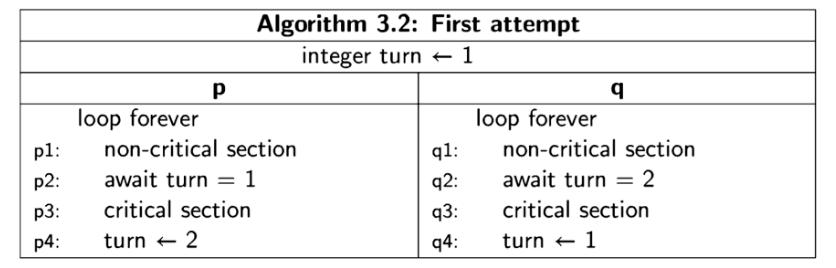
\includegraphics[width=1\textwidth]{3.2.png}\end{center}
Questo primo algoritmo propone la mutua esclusione tramite una singola variabile \textit{turn} che identifica quale processo tra \textit{p} e \textit{q} può accedere alla regione critica.
\newpage
\subsection{Rete di Petri}
In questo particolare caso è stato possibile effettuare una composizione Name-based \ref{FIG:3.2PN}.
\begin{figure*}[!ht]
\centering
\makebox[\textwidth][c]{
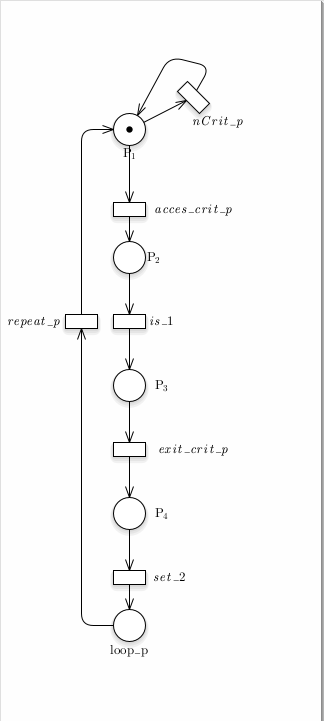
\includegraphics[width=0.5\textwidth]{p3.2.png}
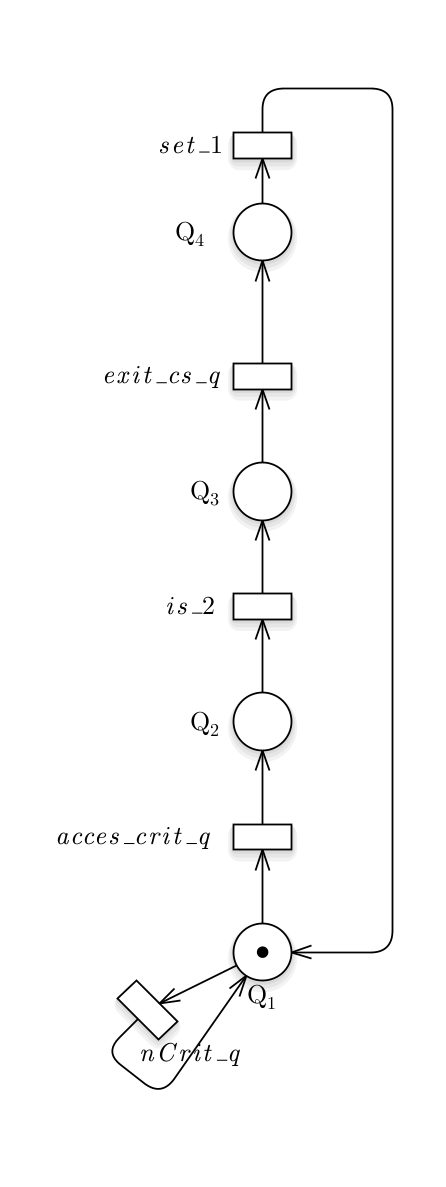
\includegraphics[width=0.5\textwidth]{q3.2.png}
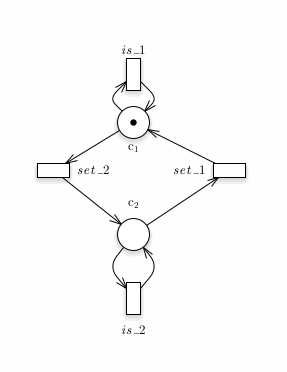
\includegraphics[width=0.5\textwidth]{variable3.2.png}}
\caption{Rete di petri decomposta} \label{FIG:decomposed3.2PN}
\end{figure*}
\begin{figure*}[!ht]
\centering
\makebox[\textwidth][c]{
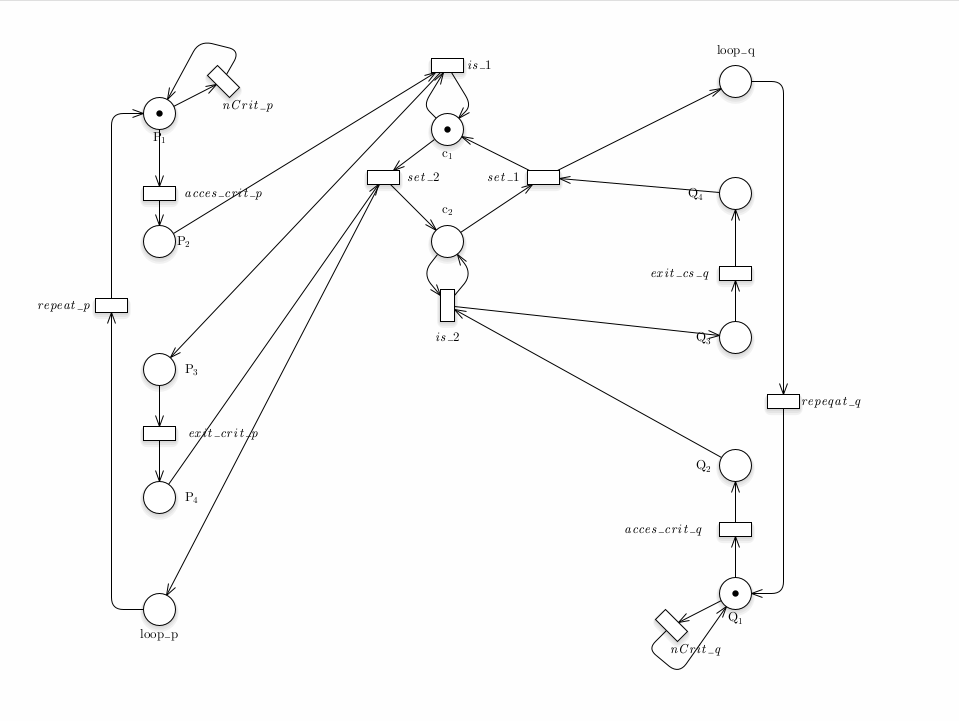
\includegraphics[width=1\textwidth]{3.2PN.png}}
\caption{Rete di petri composta} \label{FIG:3.2PN}
\end{figure*}
\newpage
\subsubsection{RG}
Il reachability graph, in figura \ref{FIG:3.2RG}, è composto da 30 stati raggiungibili e non presenta alcun deadlock.
\begin{figure*}[!ht]
\centering
\makebox[\textwidth][c]{
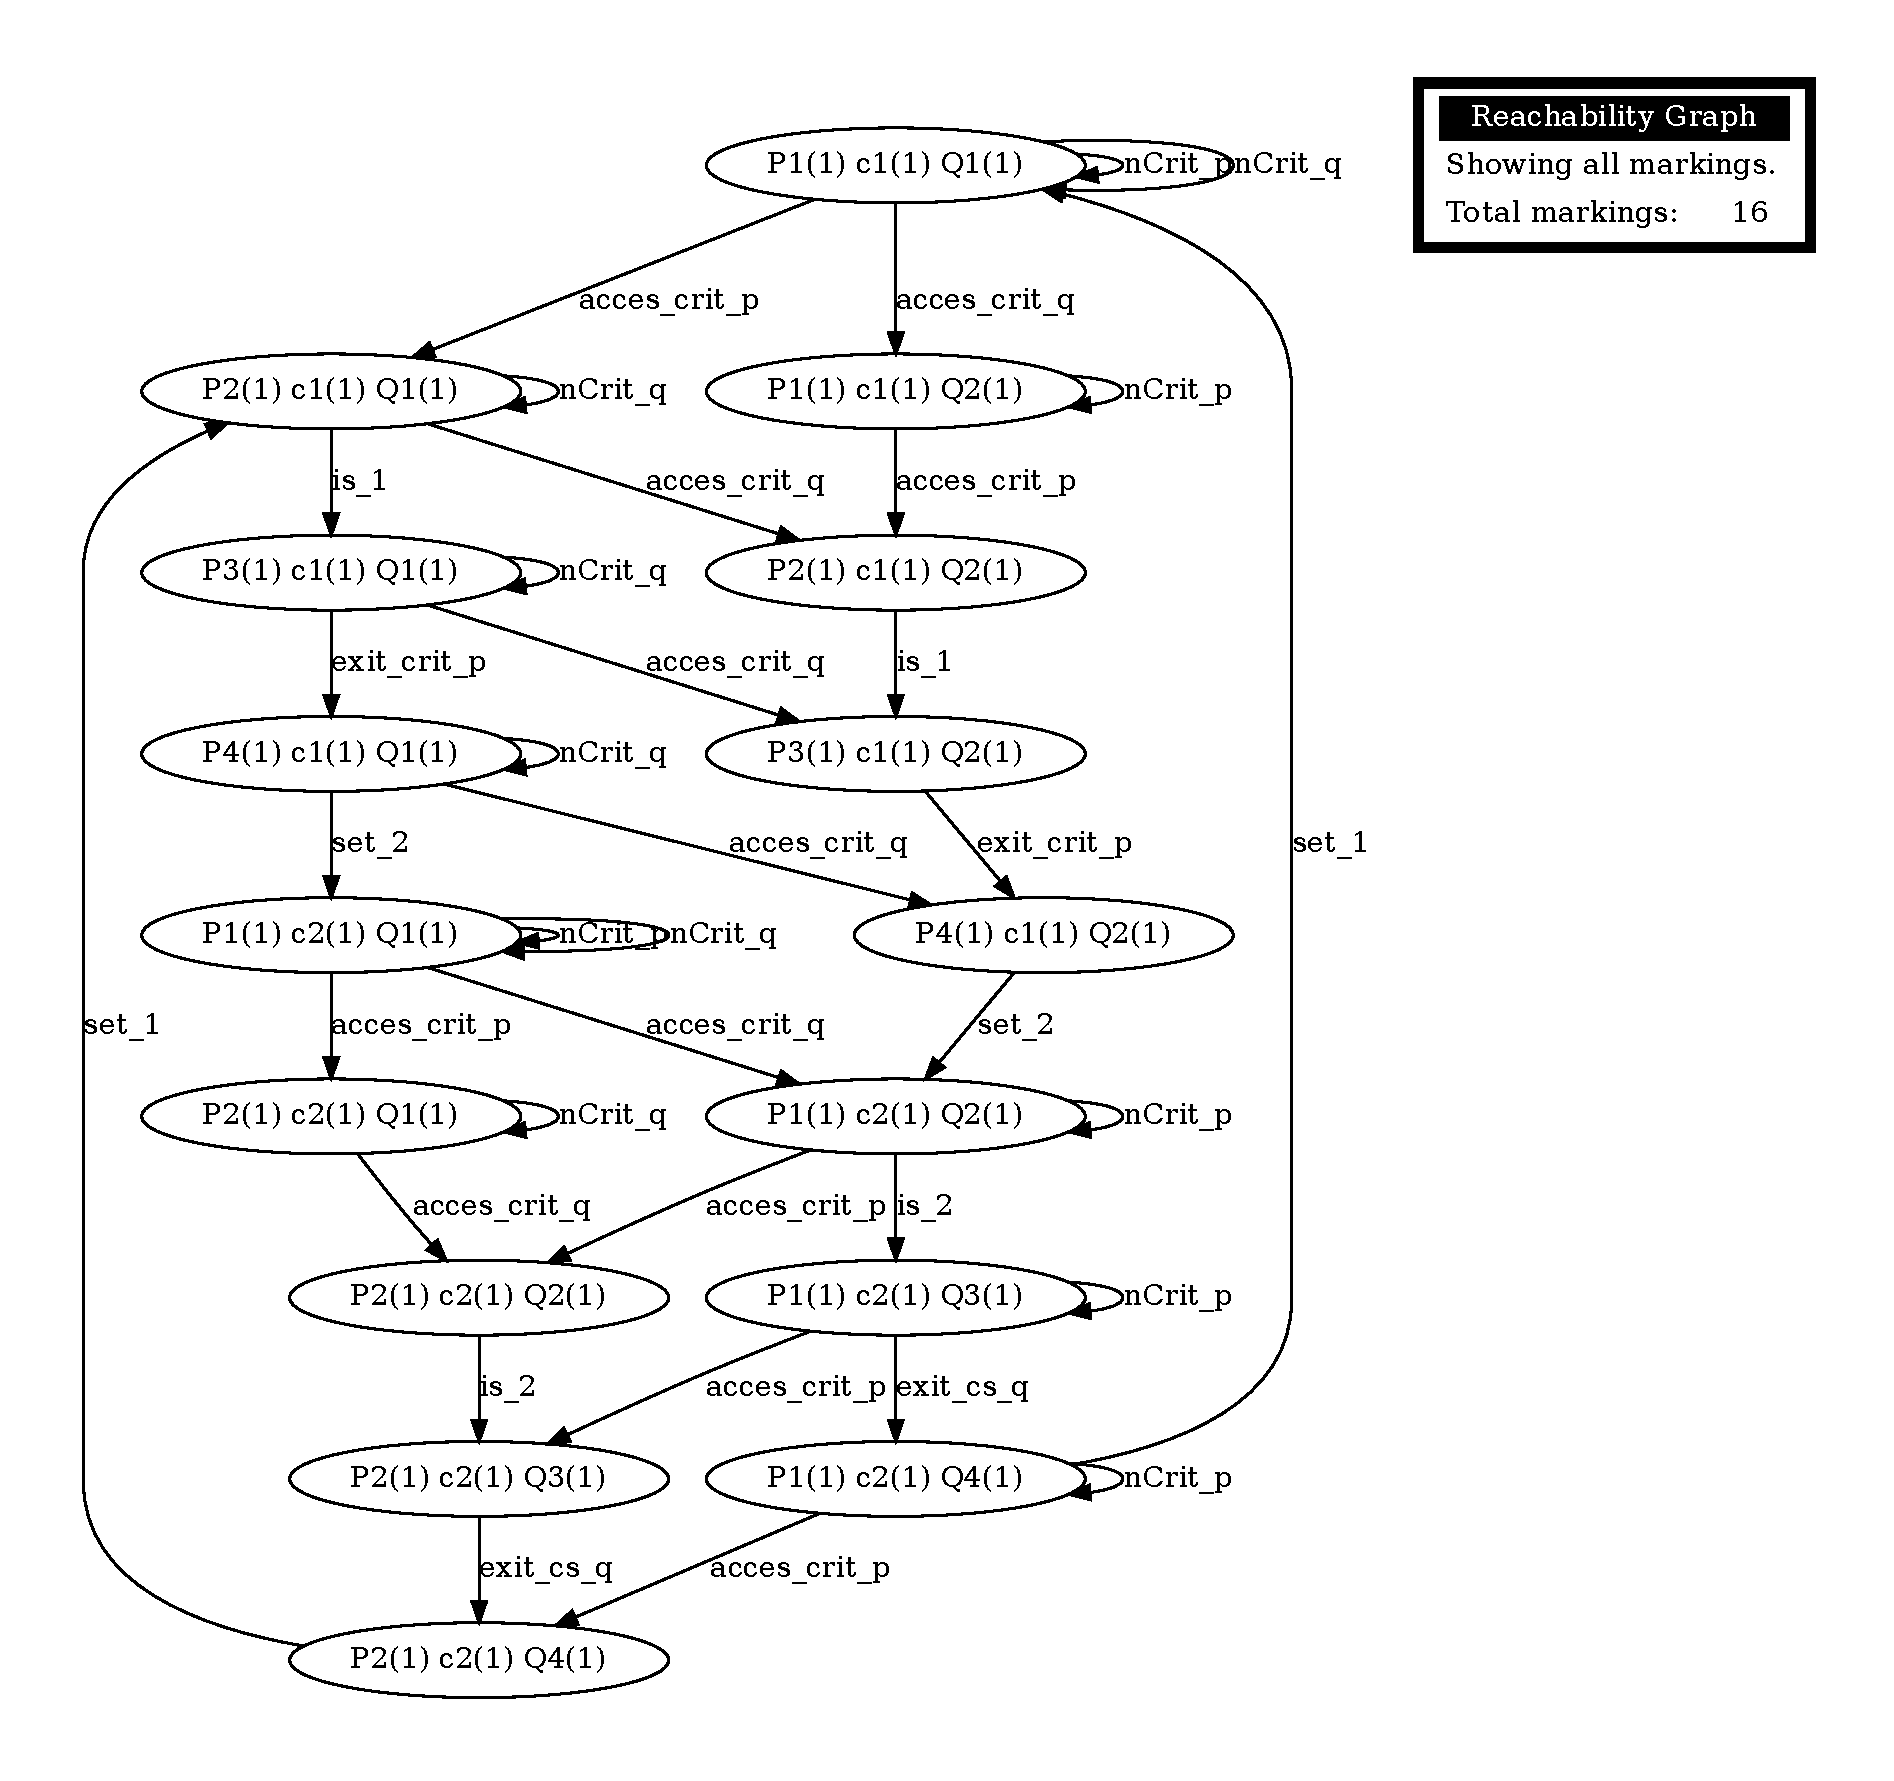
\includegraphics[width=1\textwidth]{3.2RG}}
\caption{Reachability graph 3.2} \label{FIG:3.2RG}
\end{figure*}
\newpage
\subsubsection{Analisi strutturale}
Il calcolo dei \textit{semiflow} fornisce 3 \textit{T-semiflow} minimali e 3 \textit{P-semiflow} minimali, i 3 \textit{P-semiflow} permettono di produrre dei P-invarianti e di studiare la boundedness, che in questo caso rivela che tutti i posti sono 1-bound.
Invece dallo studio dei \textit{T-semiflow} si può affermare che il sistema possiede la proprietà di \textit{liveness} in quanto è possibile individuare una \textit{firing sequence} attivabile dalla marcatura iniziale che riporta ad una situazione analoga alla situazione iniziale.
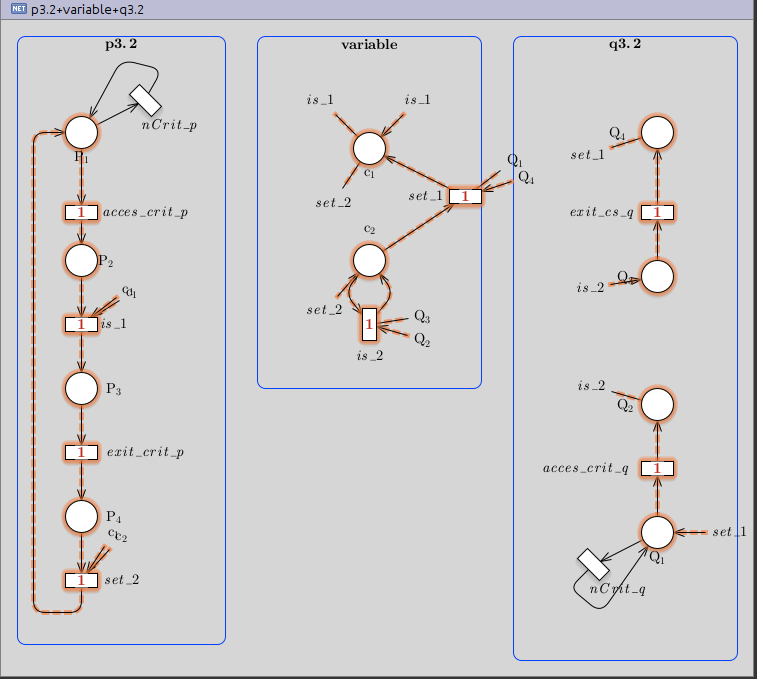
\includegraphics[width=1\textwidth]{3.2T.png}

\subsubsection{Model Checking GreatSPN}
Sono state verificate le seguenti formule CTL:
\begin{itemize}
	\item mutua esclusione: \textit{AG !(\#P3==1 \&\& \#Q3==1)} \textcolor{green}{true}.
	\item assenza di starvation: \textit{AG((\#P2 >0 ) -> (AF i\#P3>0 ))} ed anche \textit{AG((\#P2 >0 ) -> (AF i\#P3>0 ))}. Entrambe risultano \textcolor{red}{false}.\\
		Anche inserendo i fairness constrain \textit{\#P1 >0 \textit{e} \#Q1 >0} non è garantita l'assenza di starvation. Il model checker fornisce come controprova il caso in cui p è fermo al posto 2, la variabile turn vale 2 e q cicla all'infinito in sezione non critica.\\
		L'unico constrain che garantirebbe l'assenza di starvation sarebbe \textit{\#P2 >0 \textit{e} \#Q2 >0} cioè l'imposizione di progresso in regione non critica.
	\item deadlock: \textit{AG AF ((\#P1==1) || (\#Q1 == 1))} \textcolor{green}{true}. Come ci aspettavamo dalle analisi strutturali e dal DG il sistema non va in deadlock.
\end{itemize}
Sono state verificate le seguenti formule LTL:
\begin{itemize}
	\item mutua esclusione: \textit{G !(\#P3==1 \&\& \#Q3==1)} \textcolor{green}{true}.
	\item assenza di starvation: \textit{G F (\#P2==1) -> G F(\#P3 == 1)} ed anche \textit{G F (\#Q2==1) -> G F(\#Q3 == 1)}. Entrambe risultano \textcolor{red}{false}.\\
	\item deadlock: \textit{G F( (\#P1 ==1) ||  (\#Q1 ==1))} \textcolor{green}{true}.
\end{itemize}

\subsection{Algebra dei processi}
La codifica del sistema in CCS risulta essere: 
\begin{flalign*}
	&SYS = (P_1 || Q_1 || T_1) /_{\{isT_1, setT_1, isT_2, setT_2\} }&&\\
	&P_1=ncsP.P_1 + ncsP.P_2&&\\
	&P_2=isT_1.P_3&&\\
	&P_3=csP.P_4&&\\
	&P_4=setT_2.P_4&&\\
	&Q_1=ncsQ.Q_1 + ncsQ.Q_2&&\\
	&Q_2=isT_2.Q_3&&\\
	&Q_3=csQ.Q_4&&\\
	&Q_4=setT_1.Q_4&&\\\\
	&T_1=\overline{isT_1}.T_1 + \overline{setT_2}.T_2&&\\
	&T_1=\overline{isT_2}.T_2 + \overline{setT_1}.T_1&&\\
\end{flalign*}
Da cui segue il seguente derivation graph (in cui la riduzione è omessa per chiarezza).\\
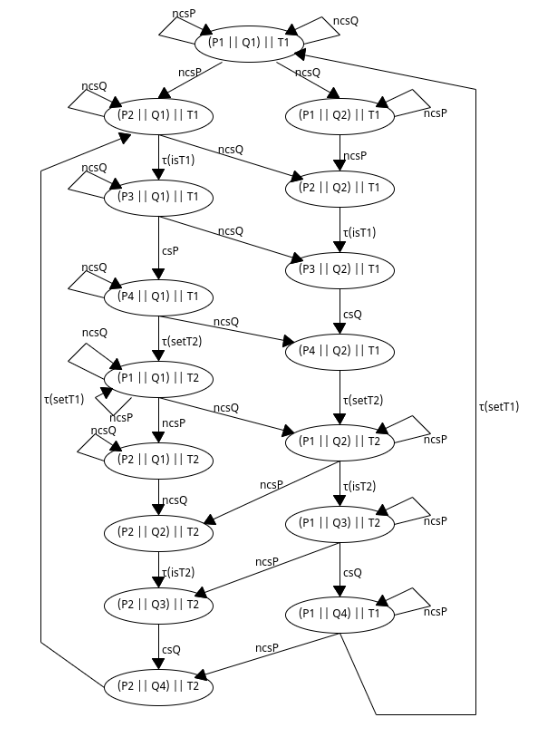
\includegraphics[width=1\textwidth]{3.2CCS.png}\\
Come si può notare il \textit{DG} è composto da 16 stati, esattamente il numero di stati raggiungibili del Reachability Graph, questo è un risultato aspettato in linea con quanto analizzato nelle corrispondenti parti dell'esercizio produttore-consumatore.

\subsection{NuSMV}
L'implementazione del sistema tramite il linguaggio di NuSMV sfrutta la similarità che c'è tra il processo P ed il processo Q.
Infatti i due programmi svolgono le stesse identiche operazioni, ma su variabili differenti, quindi basta dichiare i processi andando ad inserire correttamente i parametri.
Quindi ad esempio il processo p avrà 4 stati: lo stato s1 da cui potrà proseguire richiedendo la sezione critica, oppure rimanendo in s1, lo stato s3 che corrisponde alla sezione critica e lo stato s4 che corrisponde all'uscita dalla sezione critica ed la ripetizione del programma completo.\\
Più interessante è lo stato s4, dove si nota il riuso del codice. 
Per poter accede alla sezione critica il turno deve essere 1, quindi il processo P va a confrontare il valore della variabile \textit{turn} con lo il valore della variabile \textit{var\_wait} che in questo caso è 1, se corrispondono il programma prosegue in s3.
Operazione simile viene effettuata quando P va ad impostare il valore della variabile \textit{turn} in uscita dalla sezione critica.
\lstinputlisting{figures/3_2_code.smv}
Il comando \texttt{print\_reachable\_states} mostra 16 stati raggiungibili di 32 possibili, in linea con la dimensione del Derivation Graph e del Reachability Graph.
Tra tutti gli stati raggiungibili non è presente alcuno stato di Deadlock.

\subsubsection{Model Checking NuSMV}
Sono state verificate le seguenti formule CTL:
\begin{itemize}
        \item mutua esclusione: \textit{AG !(( p.state = s3 ) \& (q.state = s3 ))} \textcolor{green}{true}.
        \item assenza di starvation: \textit{AG (( p.state = s2 ) -> (AF p.state = s3 ))} ed anche \textit{AG (( q.state = s2 ) -> (AF q.state = s3 ))}. Entrambe risultano \textcolor{red}{false}.\\
                Anche inserendo il fairness constrain \textit{FAIRNESS running} non è garantita l'assenza di starvation. Il model checker fornisce come controprova il caso in cui p è fermo allo stato s2, la variabile turn v
ale 2 e q cicla all'infinito in sezione non critica.
        \item deadlock: \textit{AG AF (( p.state = s1 )| ( q.state = s1 ))} \textcolor{green}{true}. Come ci aspettavamo dalle analisi strutturali e dal DG il sistema non va in deadlock.
\end{itemize}
Sono state verificate le seguenti formule LTL:
\begin{itemize}
        \item mutua esclusione: \textit{G !(p.state = s3 \& q.state = s3)} \textcolor{green}{true}.
        \item assenza di starvation: \textit{G (p.state = s2 ->  F p.state = s3)} ed anche \textit{G (p.state = s2 ->  F p.state = s3)}. Entrambe risultano \textcolor{red}{false}.\\
		Anche inserendo il fairness constrain \textit{FAIRNESS running} non è garantita l'assenza di starvation. Il model checker fornisce come controprova un caso più lungo del necessario in cui comunque alla fine ci si riconduce alla situazione in cui p è fermo allo stato s2, la variabile turn vale 2 e q cicla all'infinito in sezione non critica.
        \item deadlock: \textit{G F(( p.running) | ( q.running ) )} \textcolor{red}{false}. In questo caso sembra verificarsi deadlock, perchè esiste una esecuzione in cui solo il processo Main viene eseguito.\\
		Quindi il problema non è tanto la presenza di deadlock quanto l'incapacità di scrivere la formula in modo da tenere conto anche dell'esecuzione del processo Main. Non riuscendo a rifermi al modulo main dall'interno del main stesso ho "risolto" imponendo \textit{FAIRNESS running}.
\end{itemize}

\newpage
\section{Algoritmo 3.6}
\label{SEC:3.6}
\begin{center}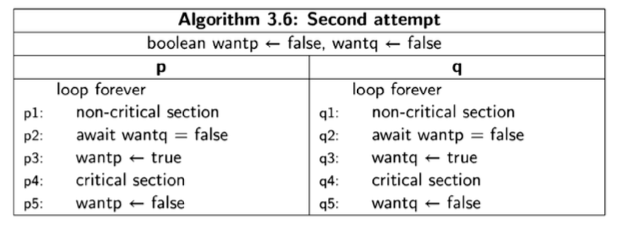
\includegraphics[width=1\textwidth]{3.6.png}\end{center}
Questo algoritmo propone la mutua esclusione tramite due variabili \textit{wantp \textit{e} wantq} che indicano se un processo vuole entrare in sezione critica. Un processo può entrare in sezione critica solamente se l'altro non vuole. quando il processo entra in sezione critica imposta la variabile relativa a lui a true. 
\subsection{Rete di Petri}
\newpage
\begin{center}
\makebox[\textwidth][c]{
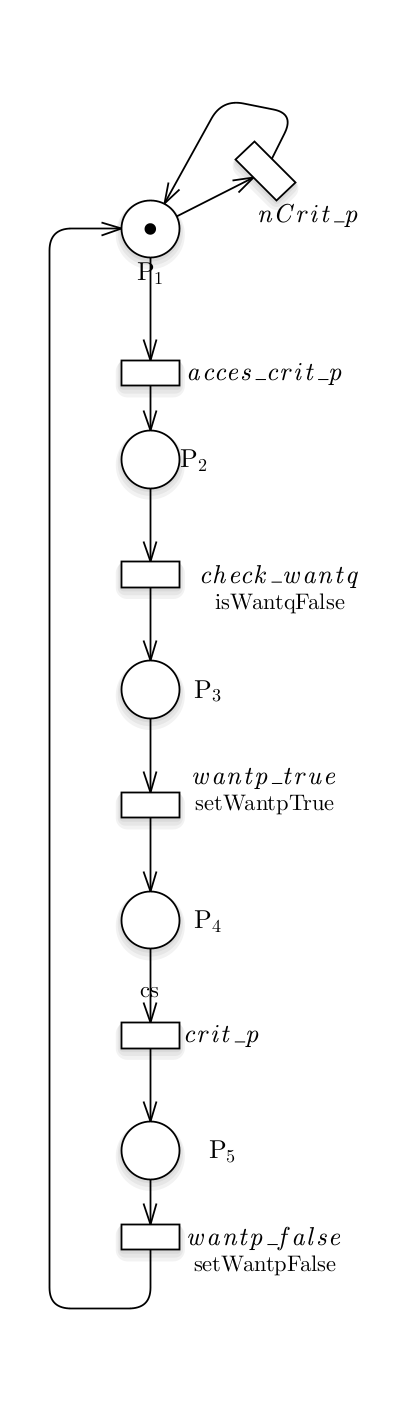
\includegraphics[width=0.34\textwidth]{p3.6.png}
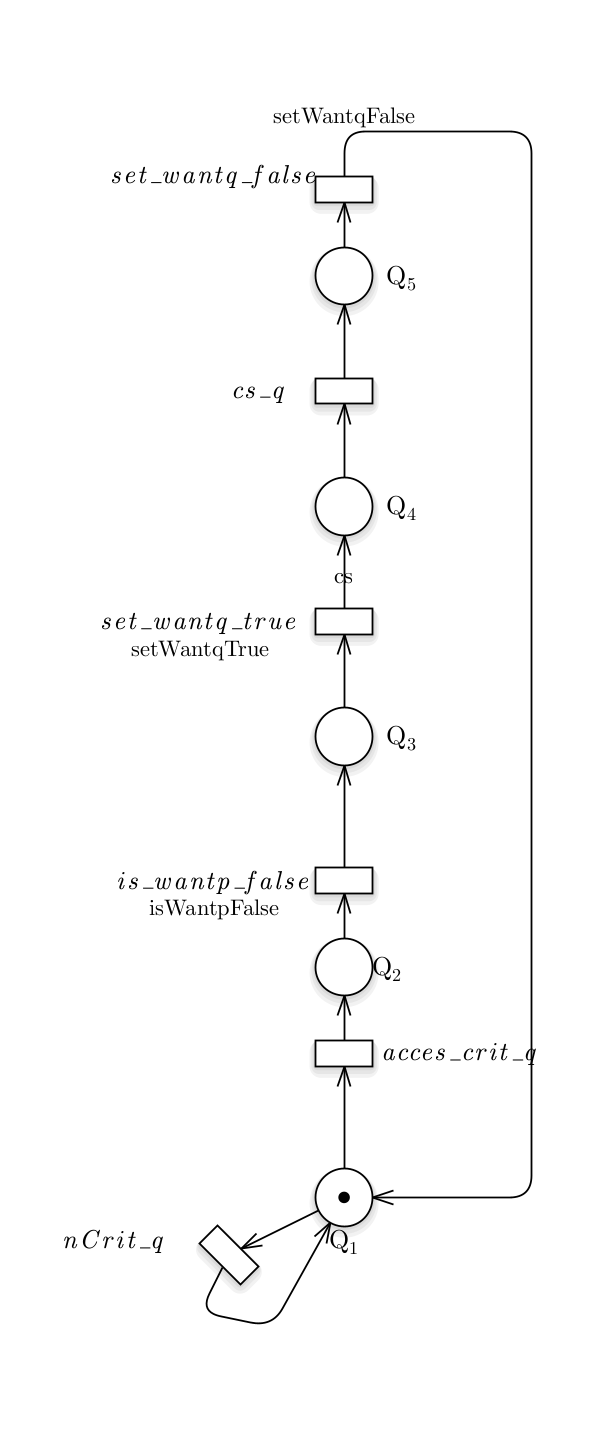
\includegraphics[width=0.5\textwidth]{q3.6.png}
}
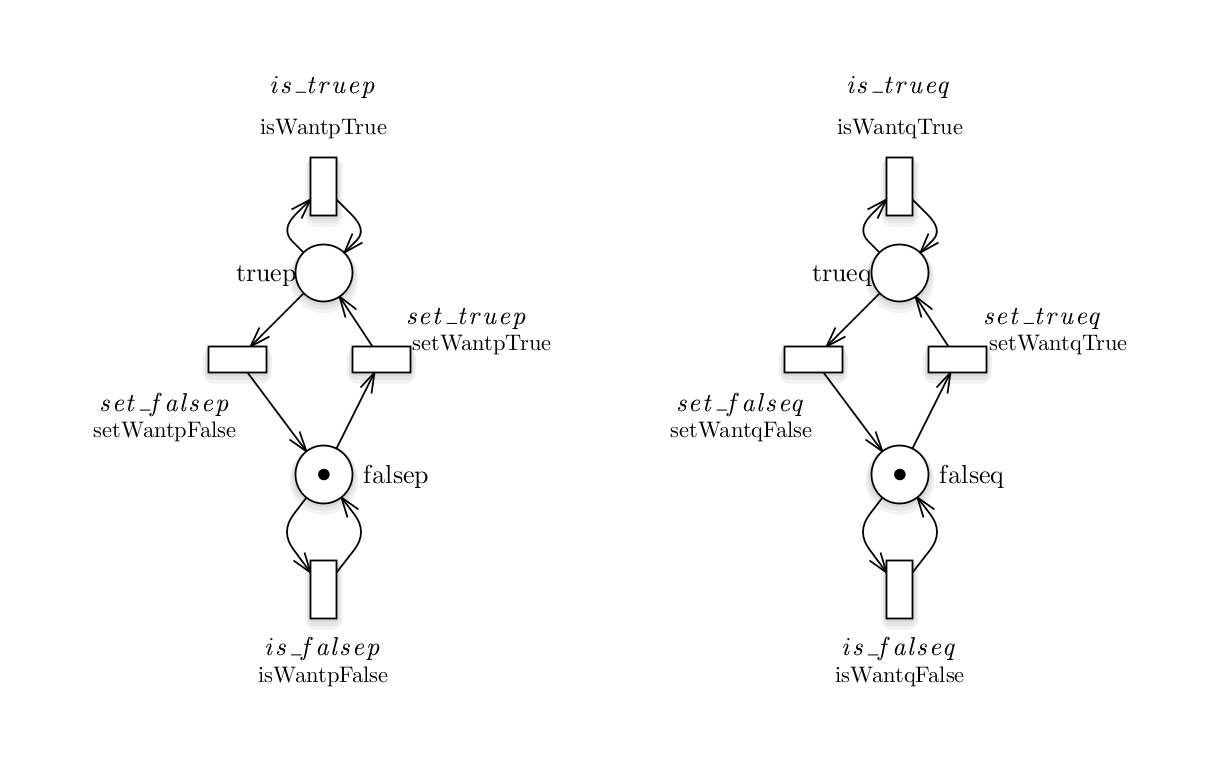
\includegraphics[width=0.8\textwidth]{variables.png}
\end{center}
\newpage
\begin{figure*}[!ht]
\centering
\makebox[\textwidth][c]{
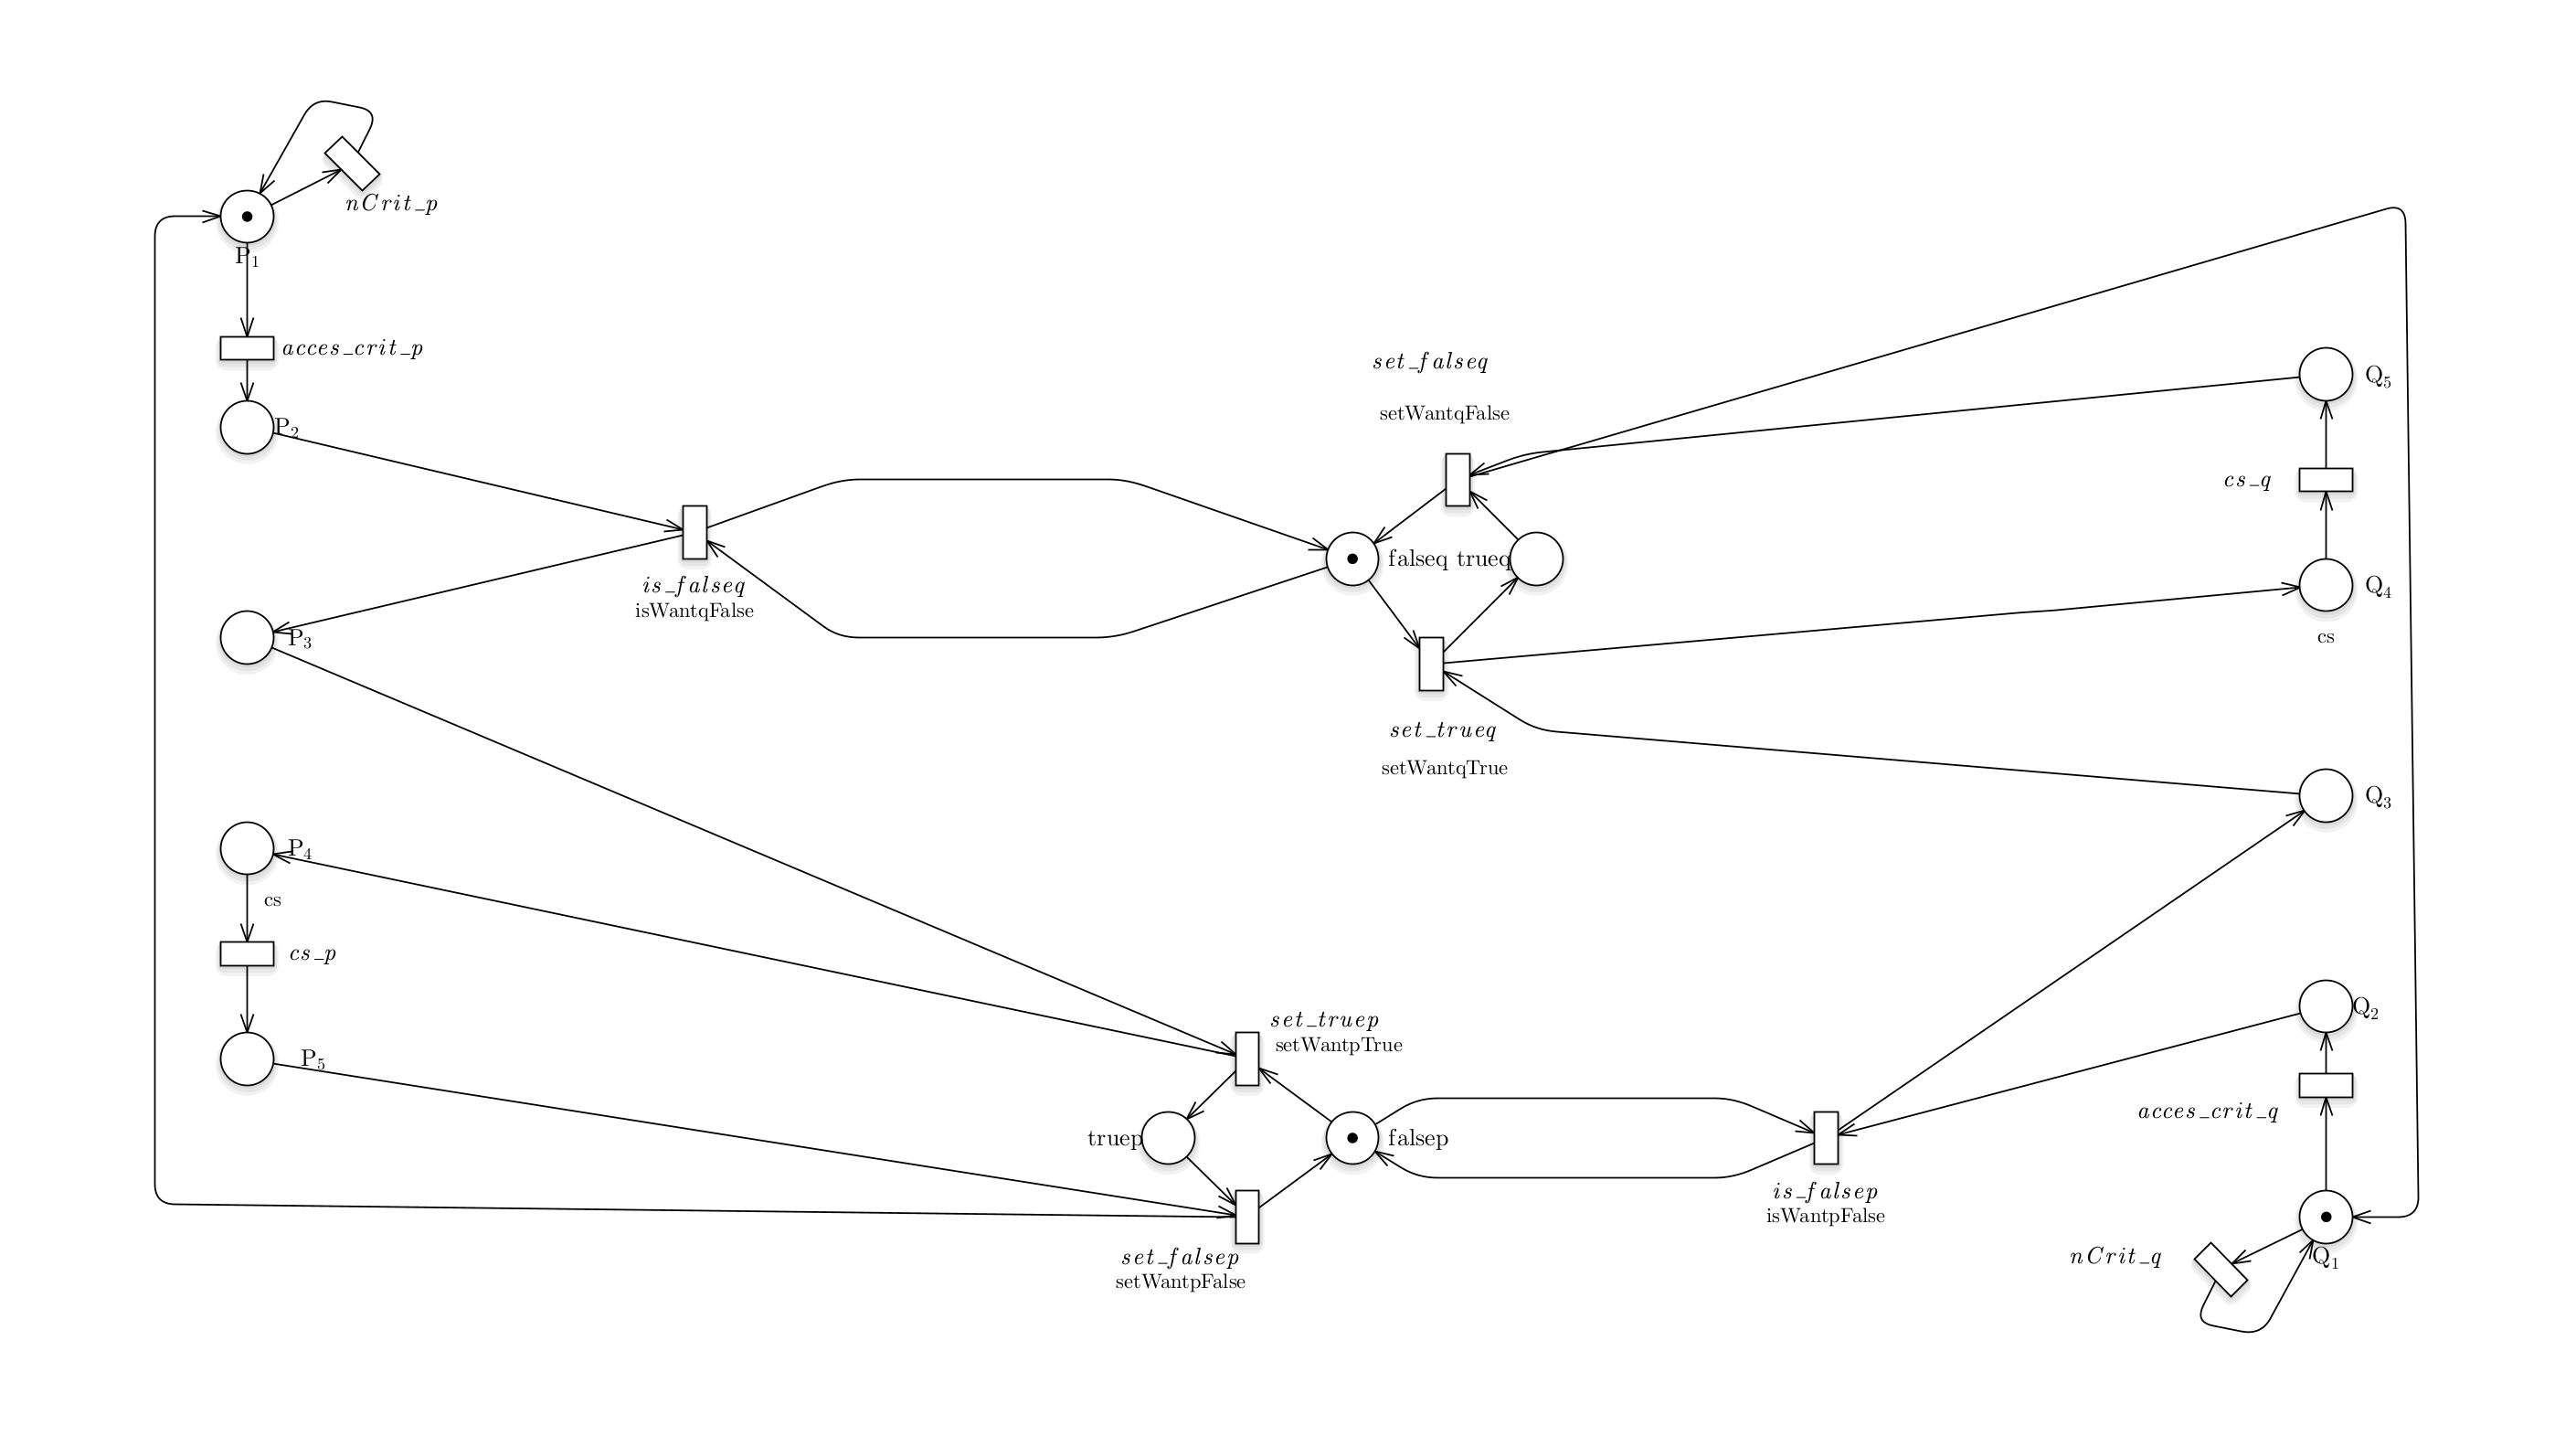
\includegraphics[width=1.6\textwidth]{3.6PN.png}}
\caption{Rete di petri composta} \label{FIG:3.6PN}
\end{figure*}
\newpage
\subsubsection{RG}
Il reachability graph, in figura \ref{FIG:3.6RG}, è composto da 25 stati raggiungibili e non presenta alcun deadlock.
\begin{figure*}[!ht]
\centering
\makebox[\textwidth][c]{
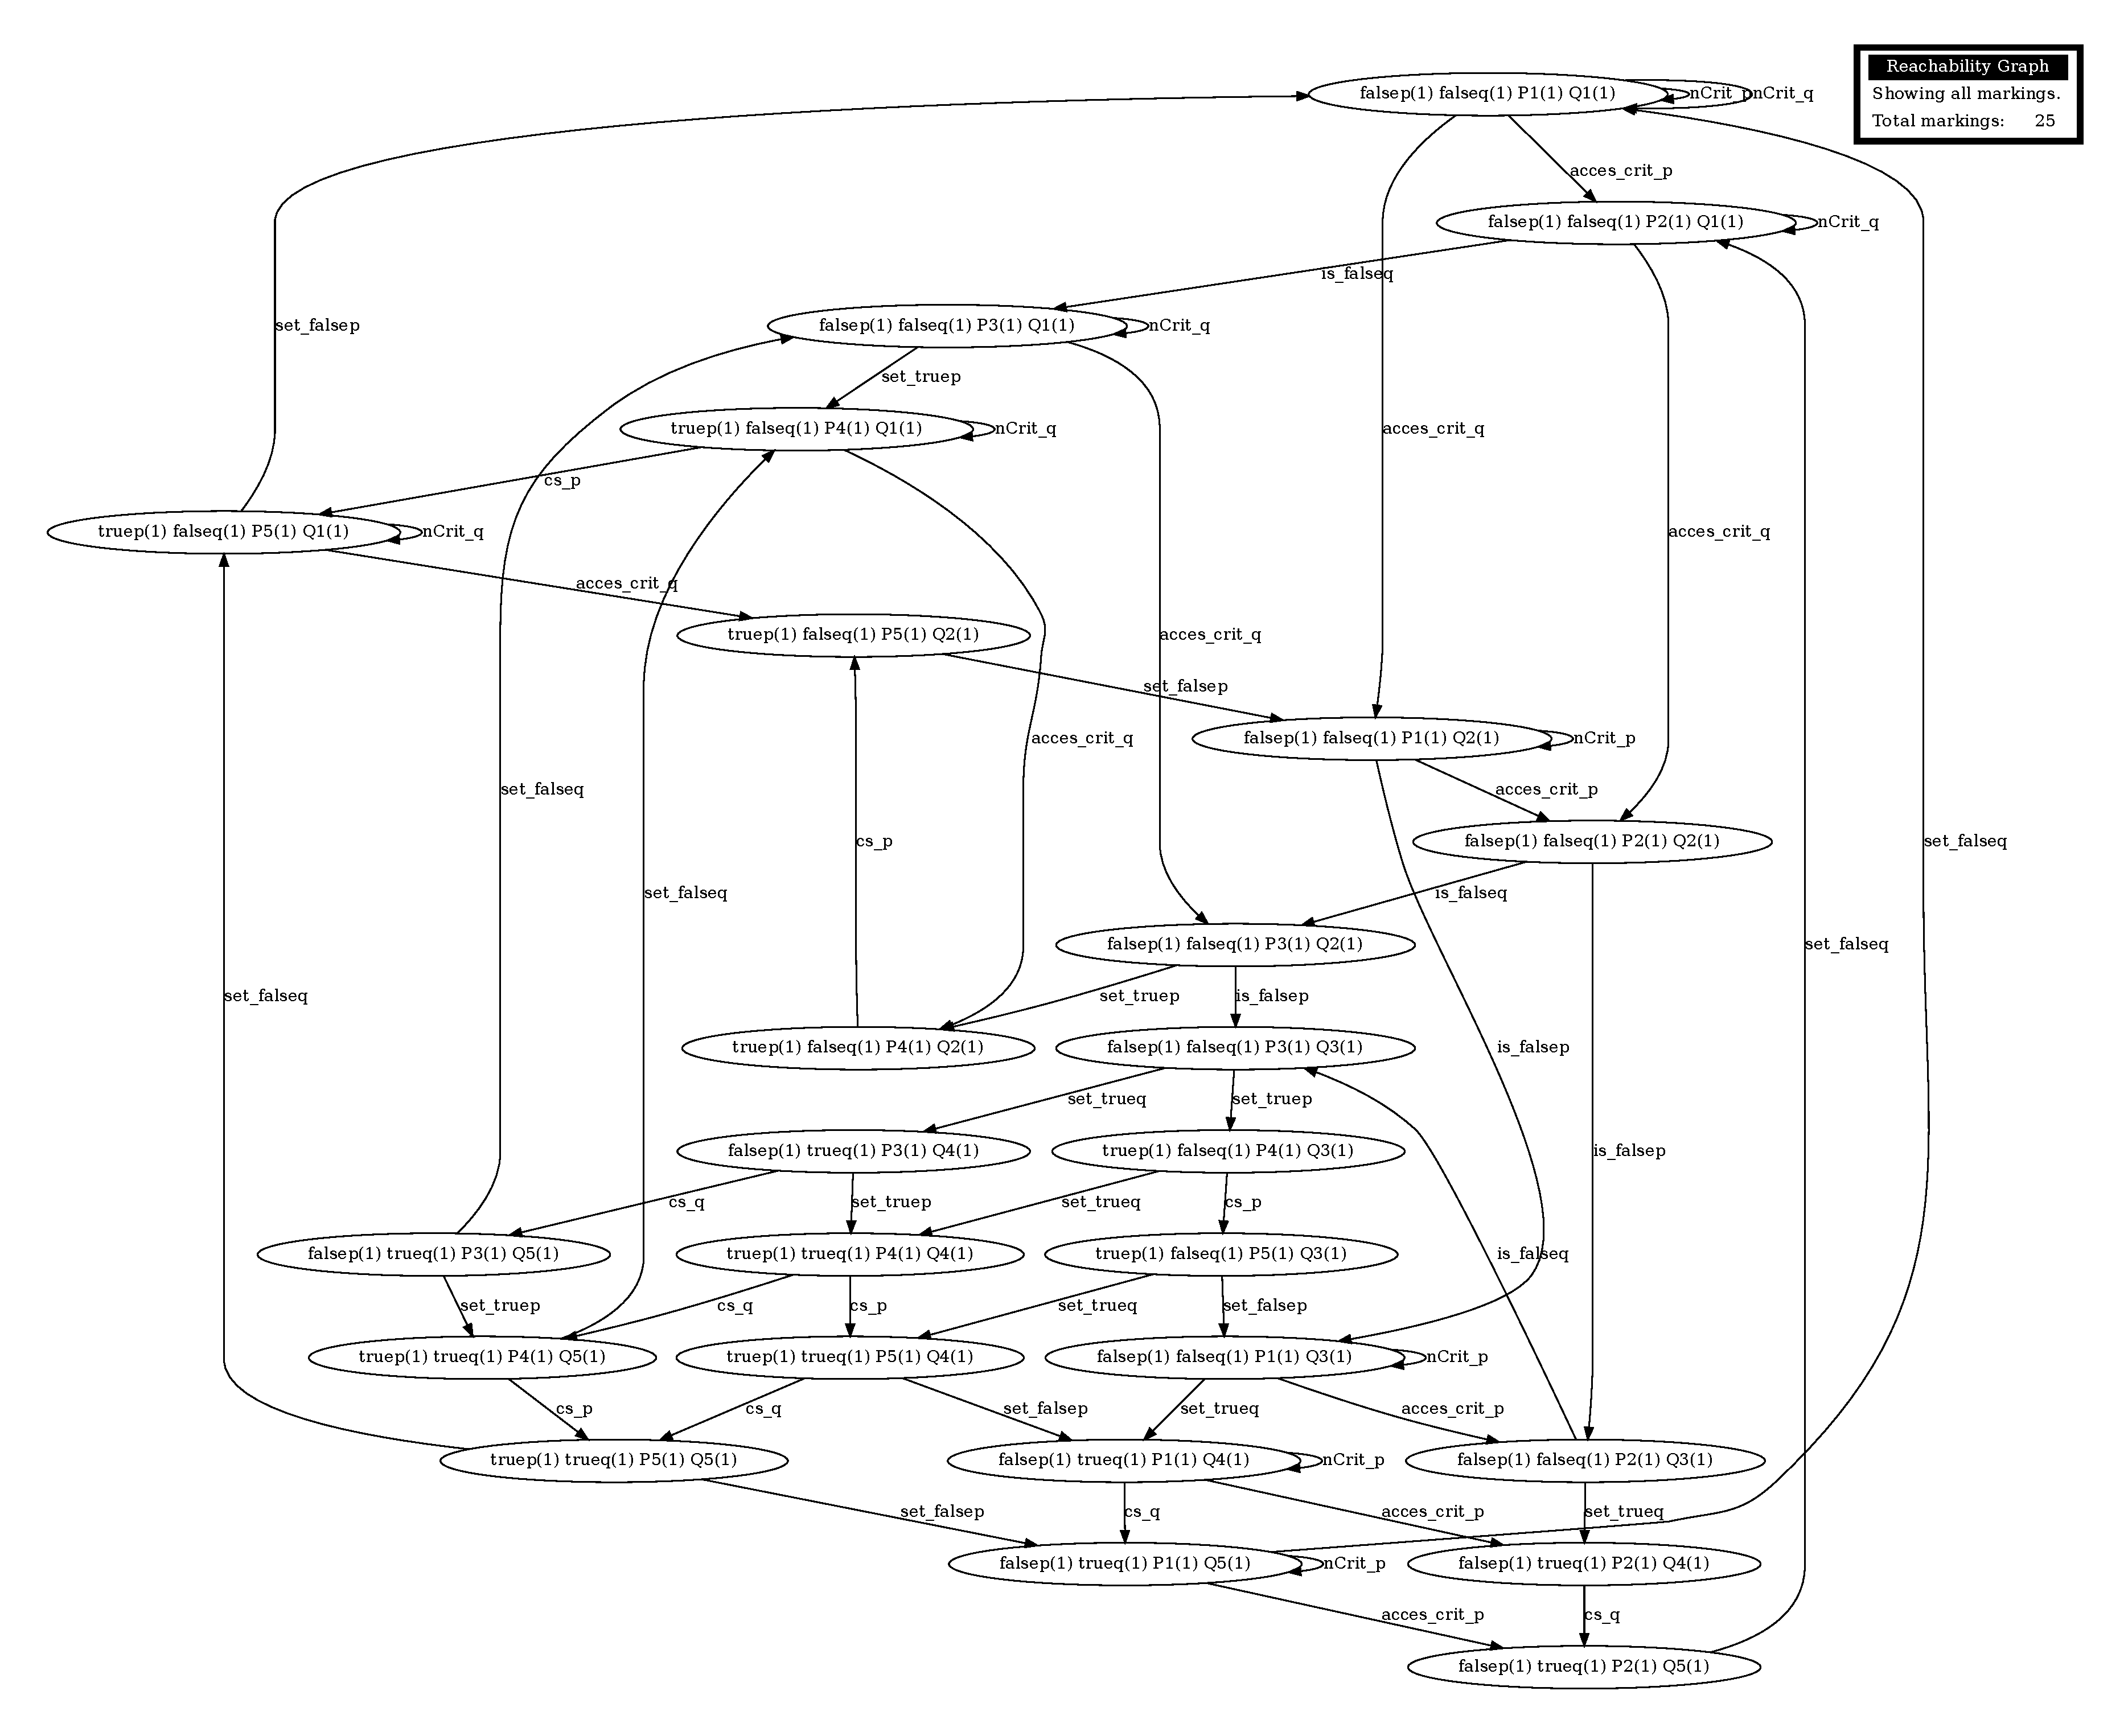
\includegraphics[width=1.5\textwidth]{3.6RG}}
\caption{Reachability graph 3.6} \label{FIG:3.6RG}
\end{figure*}
\newpage
\subsubsection{Analisi strutturale}
Il calcolo dei \textit{semiflow} fornisce 4 \textit{T-semiflow} minimali e 8 \textit{P-semiflow} minimali, gli 8 \textit{P-semiflow} permettono di produrre dei P-invarianti e di studiare la boundedness, che in questo caso rivela che tutti i posti sono 1-bound.
Invece dallo studio dei \textit{T-semiflow} si può affermare che il sistema possiede la proprietà di \textit{liveness} in quanto è possibile individuare una \textit{firing sequence} attivabile dalla marcatura iniziale che riporta ad una situazione analoga alla situazione iniziale. %TODO:
%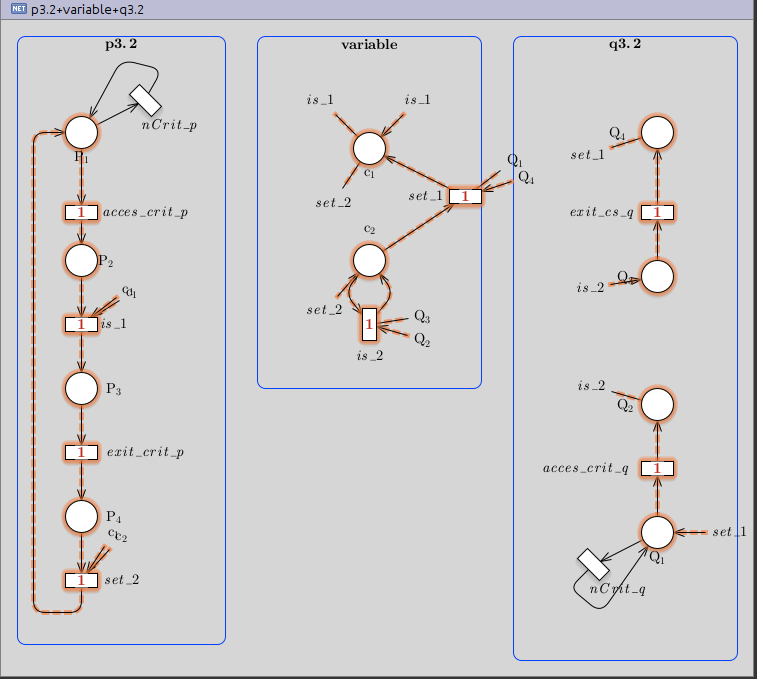
\includegraphics[width=1\textwidth]{3.2T.png}

\subsubsection{Model Checking GreatSPN}
Sono state verificate le seguenti formule CTL:
\begin{itemize}
	\item mutua esclusione: \textit{AG !(\#P4==1 \&\& \#Q4==1)} \textcolor{red}{false}.\\
		Il model checker fornisce come controesempio lesecuzione $\{P_1 Q_1,P_1 Q_2,P_2 Q_2,P_2 Q_3,P_3 Q_3,P_3 Q_4,P_4 Q_4\}$.
	\item assenza di starvation: \textit{AG((\#P2 >0 ) -> (AF i\#P4>0 ))} ed anche \textit{AG((\#P2 >0 ) -> (AF i\#P4>0 ))}. Entrambe risultano \textcolor{red}{false}.\\
		In questo caso risulta più complicato inserire dei \textit{fairness constraint} sensati. Infatti l'assenza di starvation dipende moltissimo dallo scheduling utilizzato.  
		Inserendo il fairness constrain più "elmentare", \textit{\#P1 >0 \textit{e} \#Q1 >0} cioè "viene quantomeno fornito tempo di CPU al processo p" , non è garantita l'assenza di starvation. Il model checker fornisce come controprova il caso in cui p è fermo al posto 2, e viene solo eseguito q che cicla all'infinito in sezione non critica.\\ %TODO: non sono per nulla sicuro di questa affermazione.
		Un altro constrain che garantirebbe l'assenza di starvation sarebbe \textit{\#P2 >0 \textit{e} \#Q2 >0} cioè l'imposizione di progresso in regione non critica.%TODO: non è vero e non capisco perchè
	\item deadlock: \textit{AG AF ((\#P1==1) || (\#Q1 == 1))} \textcolor{green}{true}. Come ci aspettavamo dalle analisi strutturali e dal DG il sistema non va in deadlock.
\end{itemize}
Sono state verificate le seguenti formule LTL:
\begin{itemize}
	\item mutua esclusione: \textit{G !(\#P4==1 \&\& \#Q4==1)} \textcolor{red}{false}.
	\item assenza di starvation: \textit{G F (\#P2==1) -> G F(\#P4 == 1)} ed anche \textit{G F (\#Q2==1) -> G F(\#Q4 == 1)}. Entrambe risultano \textcolor{red}{false}.\\
	\item deadlock: \textit{G F( (\#P1 ==1) ||  (\#Q1 ==1))} \textcolor{green}{true}.
\end{itemize}

\subsection{Algebra dei processi}
La codifica del sistema in CCS risulta essere: 
\begin{flalign*}
	&SYS = (P_1 || Q_1 || noWantP || noWantQ) /_{\{falseWp,falseWq,trueWp,trueWq,notWp,notWq\} }&&\\
	&P_1=ncsP.P_1 + ncsP.P_2&&\\
	&P_2=notWq.P_3&&\\
	&P_3=trueWp.P_4&&\\
	&P_4=csP.P_4&&\\
	&P_5=falseWp.P_1&&\\
	&Q_1=ncsP.P_1 + ncsP.P_2&&\\
	&Q_2=notWp.P_3&&\\
	&Q_3=trueWq.P_4&&\\
	&Q_4=csP.P_4&&\\
	&Q_5=falseWq.P_1&&\\\\
	&WantP=\overline{falseWp}.noWantP&&\\
	&noWantP=\overline{notWp}.noWantP + \overline{trueWp}.WantP &&\\
	&WantQ=\overline{falseWq}.noWantQ&&\\
	&noWantQ=\overline{notWq}.noWantQ + \overline{trueWq}.WantQ &&\\
\end{flalign*}
Da cui segue il seguente derivation graph.\\
\makebox[\textwidth][c]{
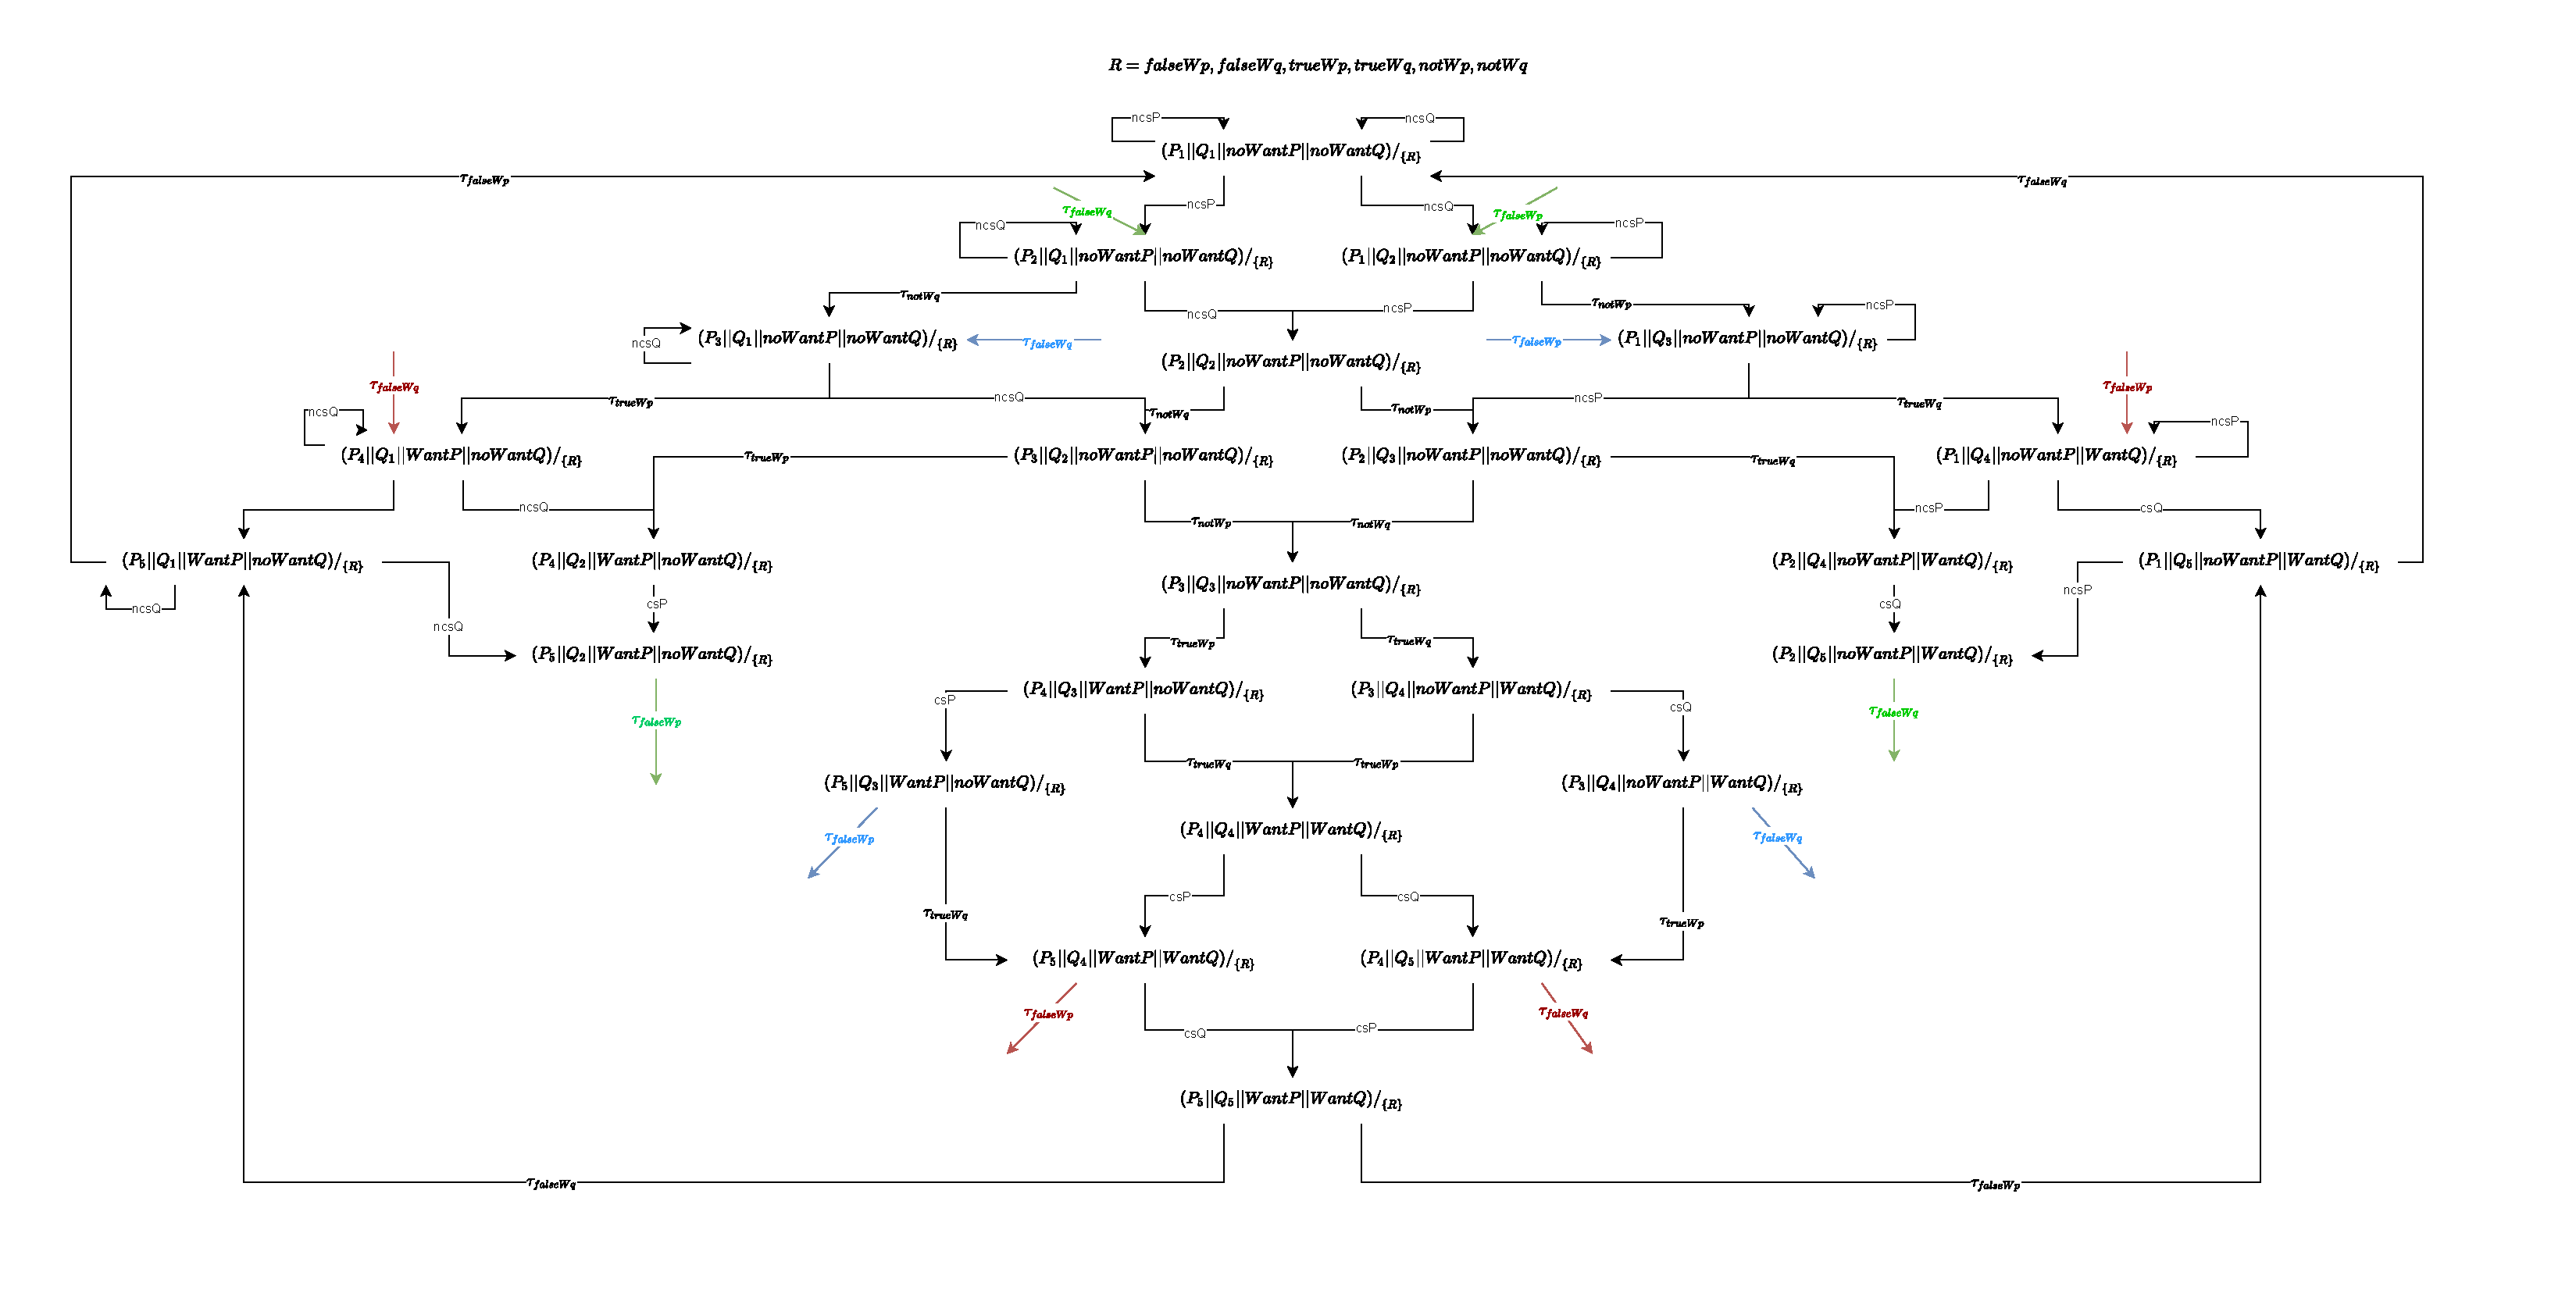
\includegraphics[width=1.5\textwidth]{3_6CCS}}\\
Come si può notare il \textit{DG} è composto da 25 stati, esattamente il numero di stati raggiungibili del Reachability Graph, questo è un risultato aspettato in linea con quanto analizzato nelle corrispondenti parti dell'esercizio produttore-consumatore.

%TODO: fare l'equivalenza tra le 2 soluzioni in PA
\subsection{NuSMV}
\label{SUBSEC:3.6NuSMV}
L'implementazione del sistema tramite il linguaggio di NuSMV sfrutta la similarità che c'è tra il processo P ed il processo Q, come nel caso precedente.
Questa volta però non è solo una variabile ad essere interessata dallo scambio di parametri, bensì le due variabili \textit{wantp} e \textit{wantq}.\\
Un paragone che rende facilmente intuibile il comportamento dei due moduli è leggere i due parametri come la variabile che indica "io voglio entrare in sezione critica" e "l'altro vuole entrare in sezione critica", ed è per questo che le due variabili sono state chiamate \textit{want\_me \textit{e} want\_other}
Per il resto il riuso del codice è identico al caso precedente.
\lstinputlisting{figures/3_6_code.smv}
Il comando \texttt{print\_reachable\_states} mostra 25 stati raggiungibili di 100 possibili, in linea con la dimensione del Derivation Graph e del Reachability Graph.
Tra tutti gli stati raggiungibili non è presente alcuno stato di Deadlock ma è presente uno stato in cui la mutua esclusione viene violata ($p.state=s4,q.state=s4,wantp=true,wantq=true$).

\subsubsection{Model Checking NuSMV}
Sono state verificate le seguenti formule CTL:
\begin{itemize}
        \item mutua esclusione: \textit{AG !(( p.state = s4 ) \& (q.state = s4 ))} \textcolor{red}{false}.\\
		Il model checker fornisce come controesempio l'esecuione $\{p.state=s1\;q.state=s1,p.state=s1\;q.state=s2,p.state=s2\;q.state=s2,p.state=s2\;q.state=s3,p.state=s3\;q.state=s3,p.state=s3\;q.state=s4,p.state=s4\;q.state=s4\}$.
        \item assenza di starvation: \textit{AG (( p.state = s2 ) -> (AF p.state = s3 ))} ed anche \textit{AG (( q.state = s2 ) -> (AF q.state = s3 ))}. Entrambe risultano \textcolor{red}{false}.\\
		Anche inserendo il fairness constrain \textit{FAIRNESS running} non è garantita l'assenza di starvation. Il model checker fornisce come controprova il caso in cui p è fermo allo stato s2, q esegue un ciclo completo del programma (tornando in s1) e 2 volte viene passata l'esecuzione al processo p. Ma p è bloccato da \textit{wantq} e non può proseguire.\\
		Questo caso specifico fa parte di una più ampia classe di esecuzioni in cui viene concessa l'esecuzione del processo p sempre quando questi è bloccato prima dell'accesso in sezione critica.
        \item deadlock: \textit{AG AF (( p.state = s1 )| ( q.state = s1 ))} \textcolor{green}{true}. Come ci aspettavamo dalle analisi strutturali e dal DG il sistema non va in deadlock.
\end{itemize}
Sono state verificate le seguenti formule LTL:
\begin{itemize}
        \item mutua esclusione: \textit{G !(p.state = s4 \& q.state = s4)} \textcolor{red}{false}.\\
		Come nel caso di CTL il sistema non rispetta la mutua esclusione, il controesempio fornito è lo stesso di CTL.
        \item assenza di starvation: \textit{G (p.state = s2 ->  F p.state = s3)} ed anche \textit{G (p.state = s2 ->  F p.state = s3)}. Entrambe risultano \textcolor{red}{false}.\\
		Anche questo caso fornisce un controesempio identico a quello fornito in fase di analisi con CTL.
        \item deadlock: \textit{G F(( p.running) | ( q.running ) )} \textcolor{red}{false}. 
		Come in sezione \ref{SEC:3.2} si pone di nuovo il problema di fare riferimento al modulo main dall'interno del modulo stesso. Viene sfruttato di nuovo \textit{FAIRNESS running} per ottenere un risultato coerente con l'analisi.
\end{itemize}

\newpage
\section{Algoritmo 3.8}
\label{SEC:3.8}
\begin{center}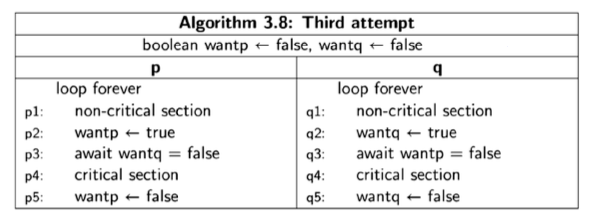
\includegraphics[width=1\textwidth]{3.8.png}\end{center}
Questo algoritmo cerca di risolvere il problema del 3.6 \ref{SEC:3.6} andando ad invertire l'operazione di setting della variabile che si riferisce al voler entrare in sezione critica e l'operazione di attesa sulla variabile che indica l'intenzione dell'altro processo
\subsection{Rete di Petri}
In questo caso è stata anche effettuata una modifica alle variabili rimuovendo le transizioni \texttt{is\_true}, in quanto nell'algoritmo 3.8 non viene mai controllato se una variabile è vera.
\newpage
\begin{center}
\makebox[\textwidth][c]{
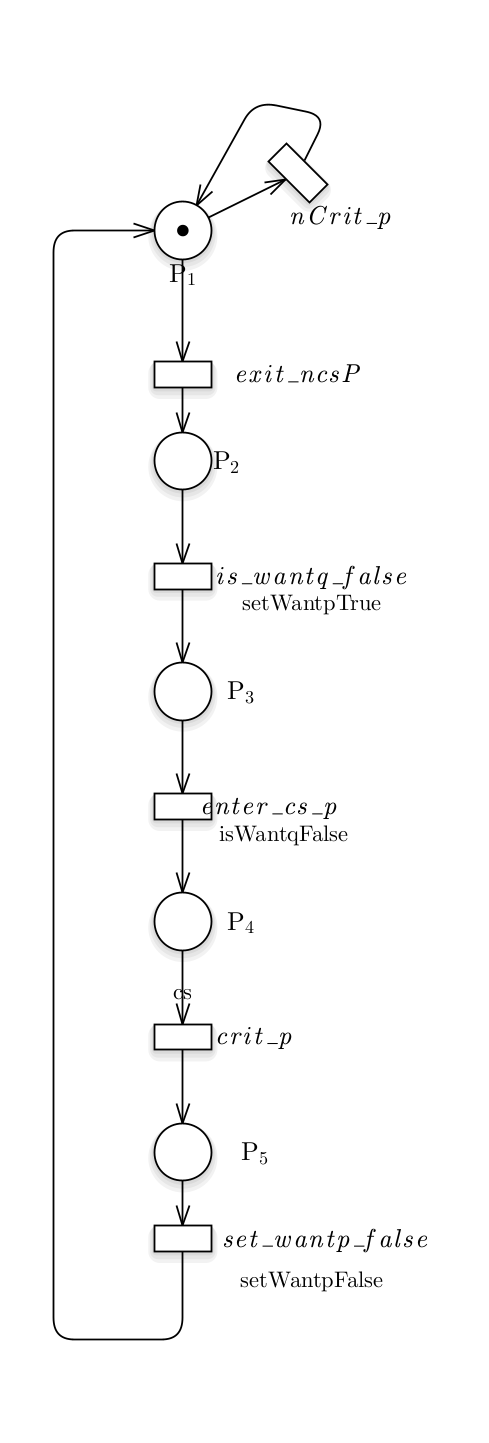
\includegraphics[width=0.4\textwidth]{p3.8.png}
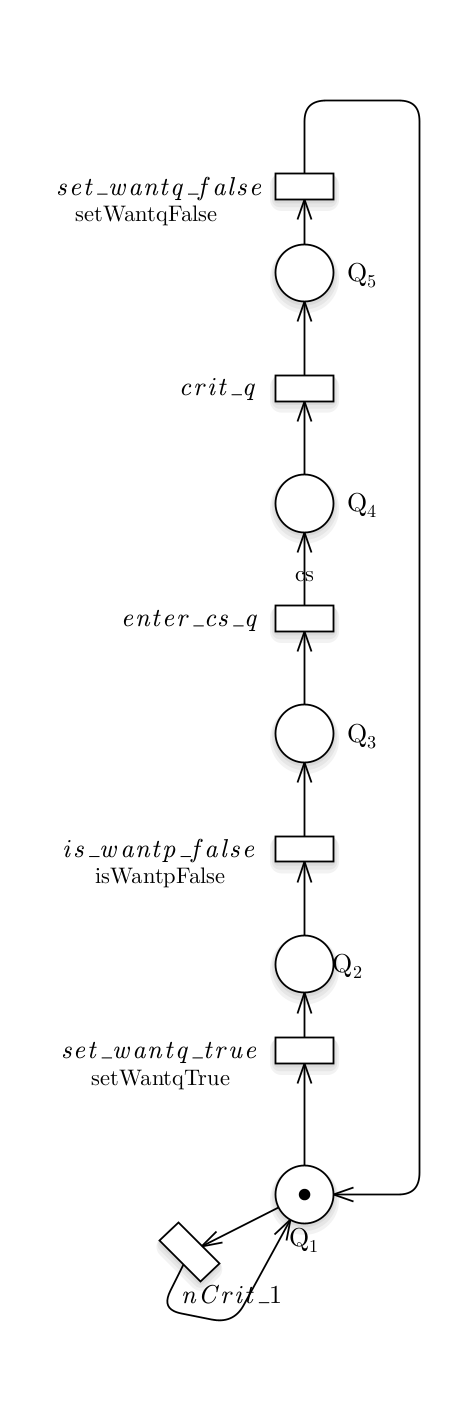
\includegraphics[width=0.4\textwidth]{q3.8.png}
}
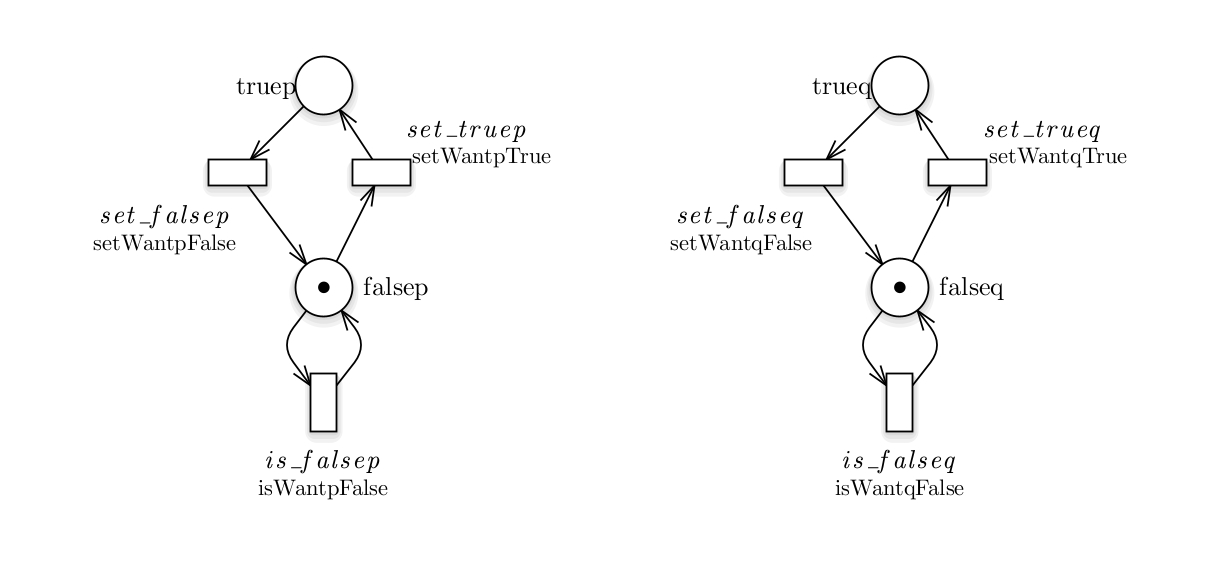
\includegraphics[width=0.8\textwidth]{variables_noTrue.png}
\end{center}
\newpage
\begin{figure*}[!ht]
\centering
\makebox[\textwidth][c]{
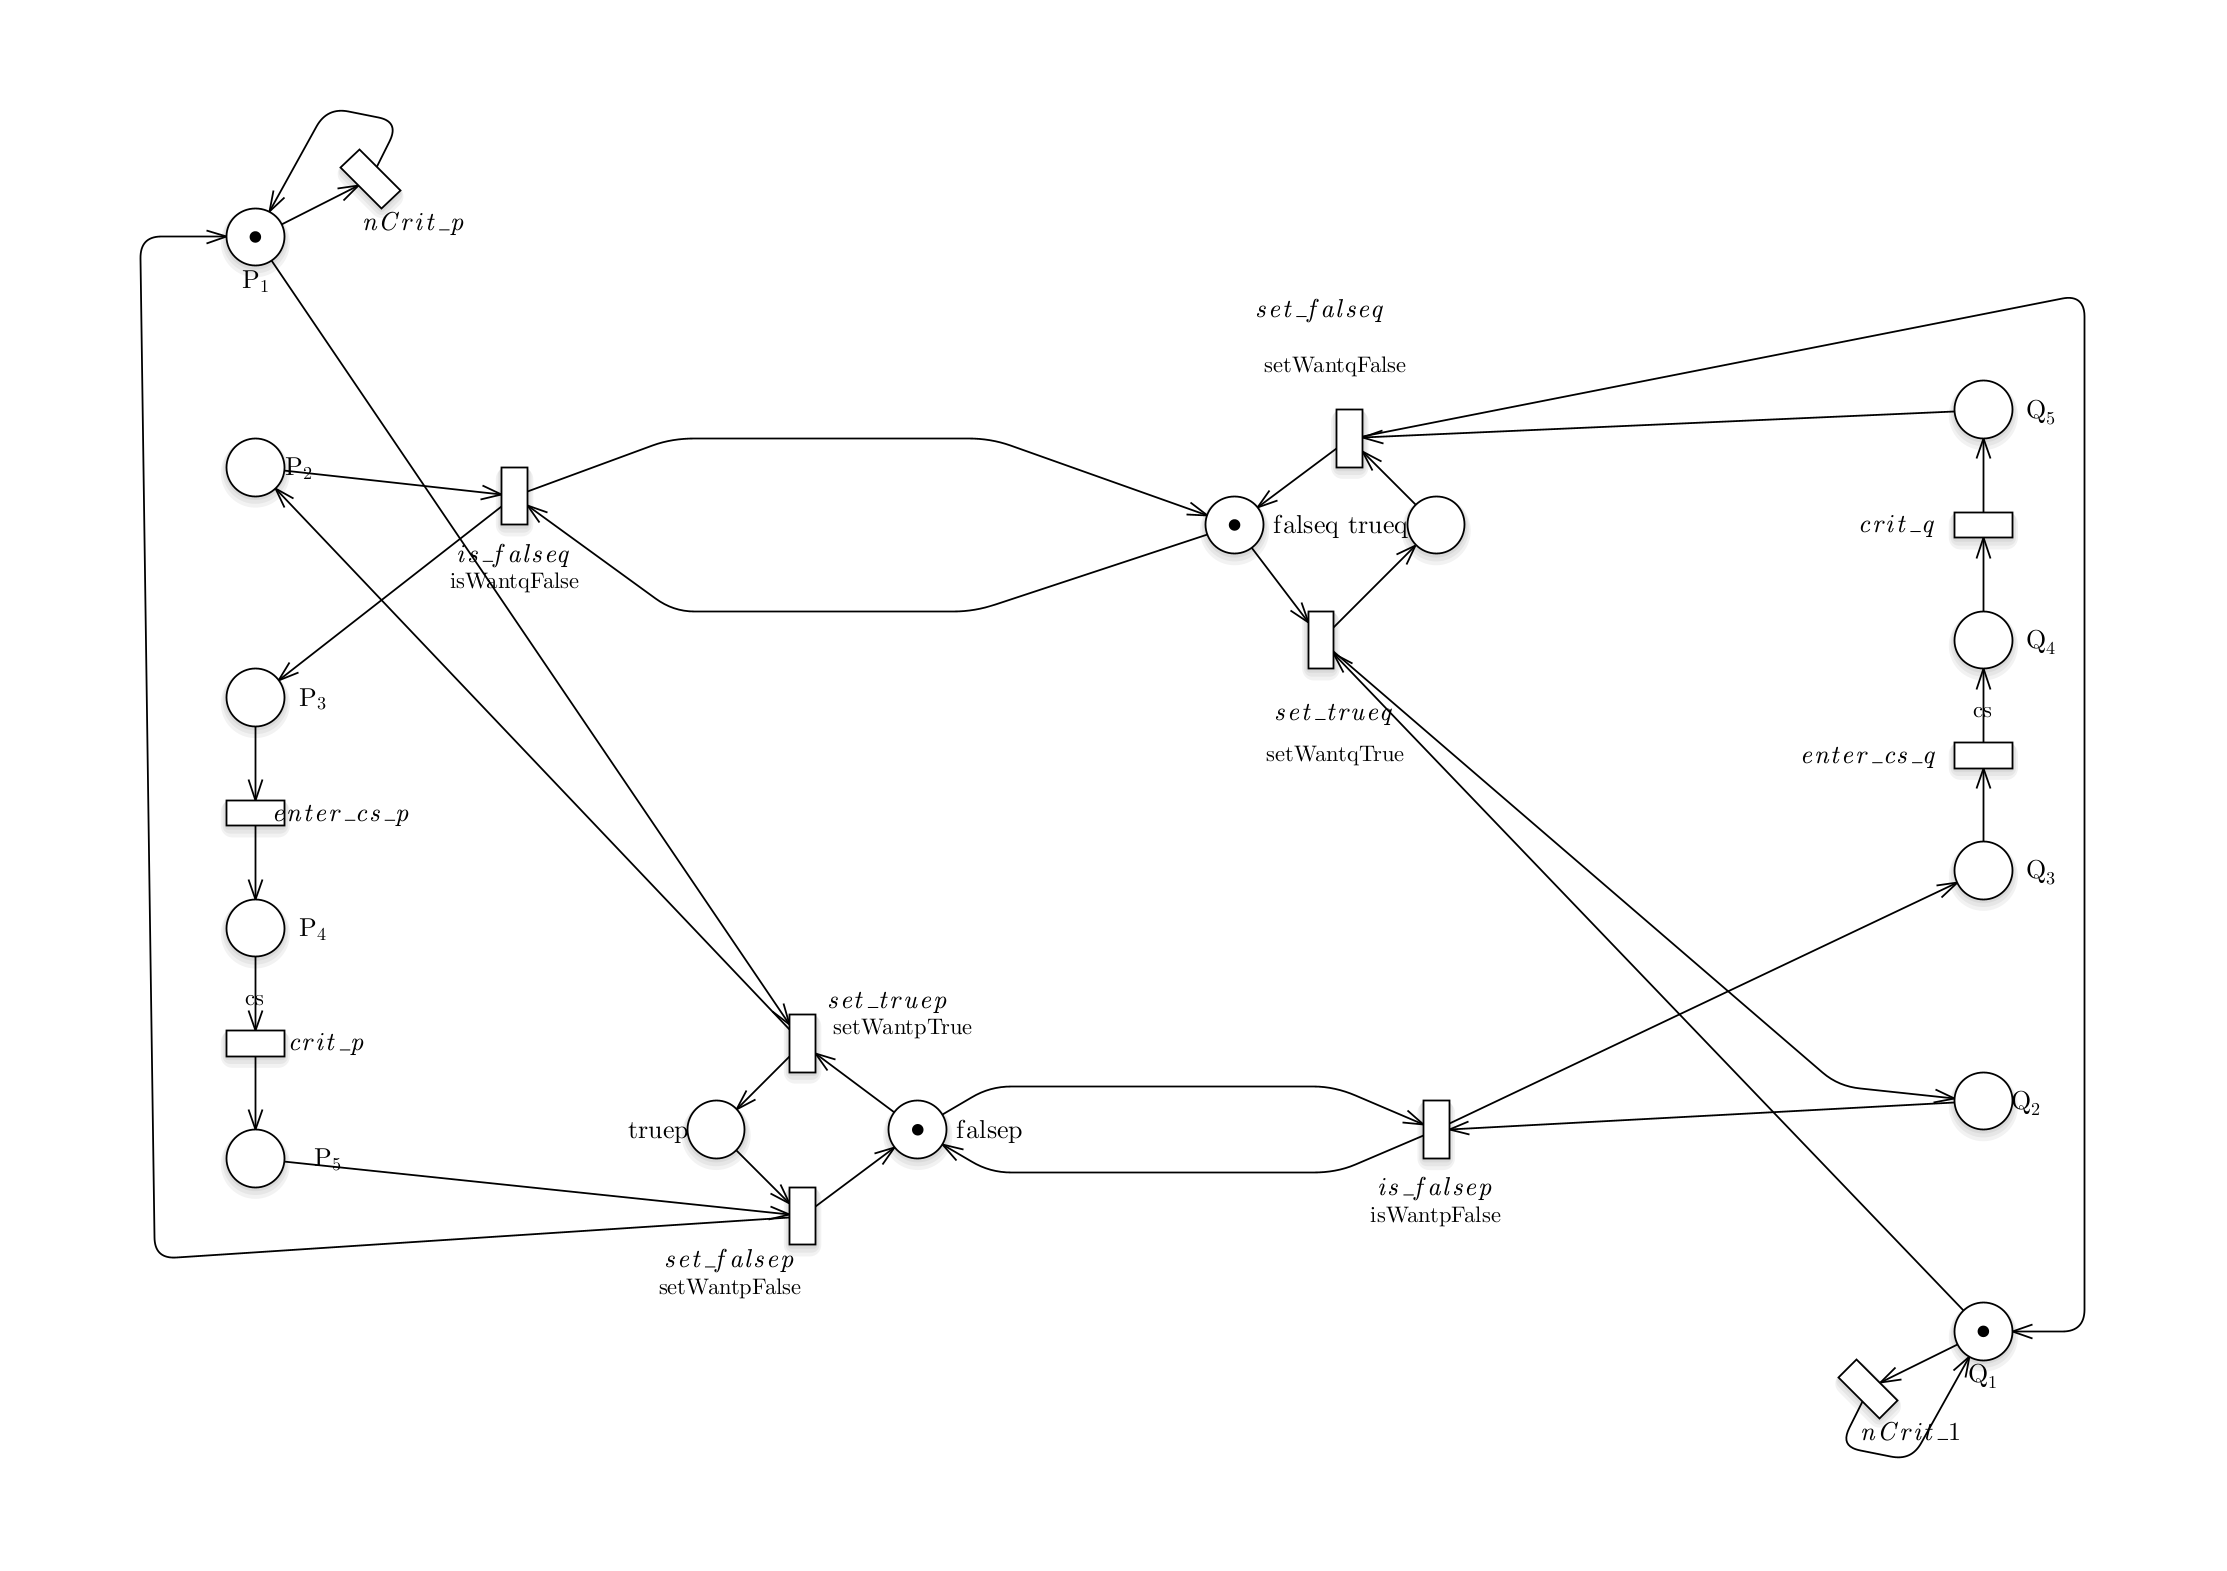
\includegraphics[width=1.6\textwidth]{3.8PN.png}}
\caption{Rete di petri composta} \label{FIG:3.8PN}
\end{figure*}
\newpage
\subsubsection{RG}
Il reachability graph, in figura \ref{FIG:3.8RG}, è composto 21 stati, di cui uno rappresentante una situazione di Deadlock.
\begin{figure*}[!ht]
\centering
\makebox[\textwidth][c]{
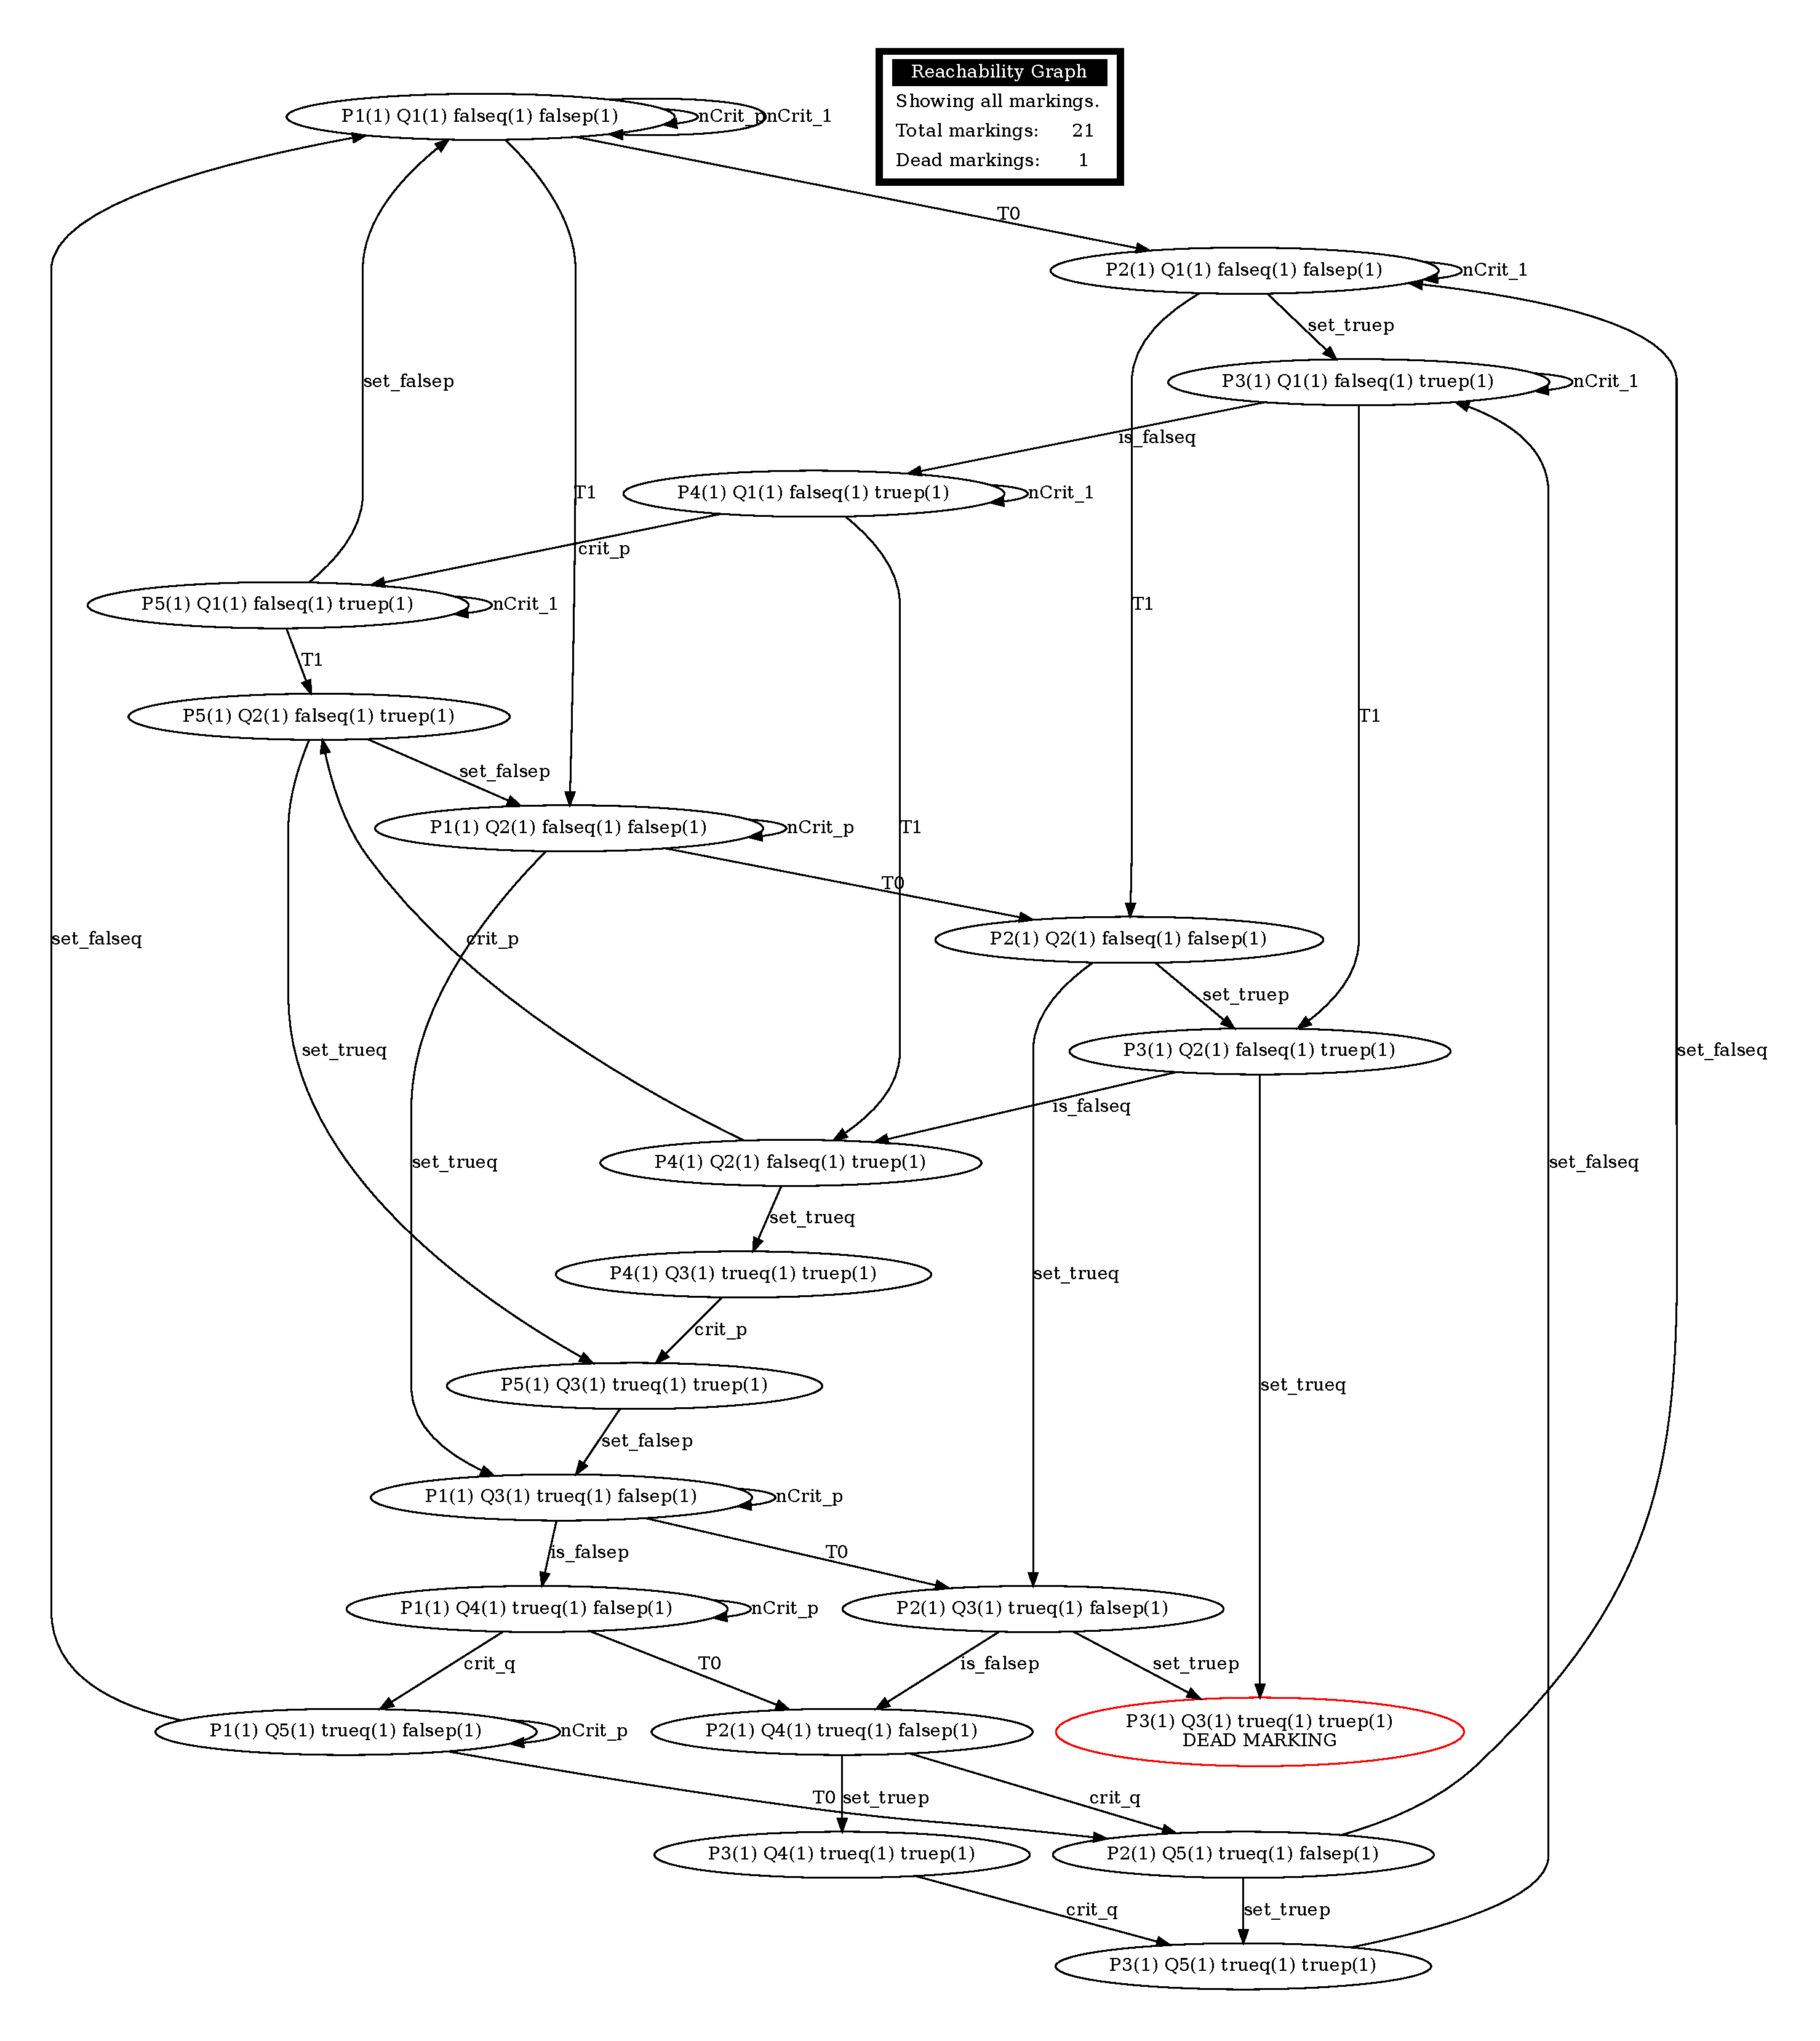
\includegraphics[width=1\textwidth]{3.8RG}}
\caption{Reachability graph 3.8} \label{FIG:3.8RG}
\end{figure*}
\newpage
\subsubsection{Analisi strutturale}

\subsubsection{Model Checking GreatSPN}
Sono state verificate le seguenti formule CTL:
\begin{itemize}
	\item mutua esclusione: \textit{AG !(\#P4==1 \&\& \#Q4==1)} \textcolor{green}{true}.\\
		Il sistema rispetta la mutua esclusione.
	\item deadlock: \textit{AG AF ((\#P1==1) || (\#Q1 == 1))} \textcolor{red}{false}.\\
		Il sistema va in deadlock, il controesempio presentato dal Model Checker è l'esecuzione $\{P_1Q_1 \rightarrow P_1Q_2 \rightarrow P_2Q_2\}$.
	\item assenza di starvation: \textit{AG((\#P2 >0 ) -> (AF i\#P4>0 ))} ed anche \textit{AG((\#P2 >0 ) -> (AF i\#P4>0 ))}. Entrambe risultano \textcolor{red}{false}.\\
		Essendoci deadlock c'è sempre la possibilità di starvation. Se il sistema va in deadlock dopo l'esecuzione del punto precedente entrambi i processi presentano starvation.
\end{itemize}
Sono state verificate le seguenti formule LTL:
\begin{itemize}
	\item mutua esclusione: \textit{G !(\#P4==1 \&\& \#Q4==1)} \textcolor{green}{true}.
	\item assenza di starvation: \textit{G F (\#P2==1) -> G F(\#P4 == 1)} ed anche \textit{G F (\#Q2==1) -> G F(\#Q4 == 1)}. Entrambe risultano \textcolor{red}{false}.\\
	\item deadlock: \textit{G F( (\#P1 ==1) ||  (\#Q1 ==1))} \textcolor{red}{false}.
\end{itemize}

\subsubsection{Riduzione}

\subsection{NuSMV}
L'implementazione del sistema tramite il linguaggio di NuSMV è pressochè identica a quella della sezione \ref{SUBSEC:3.6NuSMV}, l'unica differenza sta nella posizione del controllo \texttt{!want\_other} che questa volta viene effettuato dopo aver impostato la variabile \textit{want\_me} a true.
\lstinputlisting{figures/3_8_code.smv}
Il comando \texttt{print\_reachable\_states} mostra 21 stati raggiungibili di 100 possibili, in linea con la dimensione del Reachability Graph.
È presente uno stato di deadlock : $p.state=s3, \; q.state=s3, \; wantp = true, \; wantq = true $. 

\subsubsection{Model Checking NuSMV}
Sono state verificate le seguenti formule CTL:
\begin{itemize}
        \item mutua esclusione: \textit{AG !(( p.state = s4 ) \& (q.state = s4 ))} \textcolor{green}{true}.
        \item deadlock: \textit{AG AF (( p.state = s1 )| ( q.state = s1 ))} \textcolor{red}{false}.\\
		Il sistema va in deadlock, il controesempio presentato dal Model Checker è una esecuzione che fa eseguire tutti gli stati di q tornando a q.state= s1 e poi esegue $\{P_1Q_1 \rightarrow P_1Q_2 \rightarrow P_2Q_2\}$ che lo porta in deadlock.
        \item assenza di starvation: \textit{AG (( p.state = s2 ) -> (AF p.state = s3 ))} ed anche \textit{AG (( q.state = s2 ) -> (AF q.state = s3 ))}. Entrambe risultano \textcolor{red}{false}.\\
		Essendoci deadlock c'è sempre la possibilità di starvation. Se il sistema va in deadlock dopo l'esecuzione presentata precedente entrambi i processi presentano starvation.
		L'esempio presentato dal Model Checker è lo stesso del caso di deadlock.
\end{itemize}
Sono state verificate le seguenti formule LTL:
\begin{itemize}
        \item mutua esclusione: \textit{G !(p.state = s4 \& q.state = s4)} \textcolor{green}{true}.\\
        \item deadlock: \textit{G F(( p.running) | ( q.running ) )} \textcolor{red}{false}. \\
		Il sistema va in deadlock, il controesempio presentato dal Model Checker è una esecuzione che fa eseguire tutti gli stati di q tornando a q.state= s1 e poi esegue $\{P_1Q_1 \rightarrow P_1Q_2 \rightarrow P_2Q_2\}$ che lo porta in deadlock.
        \item assenza di starvation: \textit{G (p.state = s2 ->  F p.state = s3)} ed anche \textit{G (p.state = s2 ->  F p.state = s3)}. Entrambe risultano \textcolor{red}{false}.\\
		Essendoci deadlock c'è sempre la possibilità di starvation. Se il sistema va in deadlock dopo l'esecuzione presentata precedente entrambi i processi presentano starvation.
		L'esempio presentato dal Model Checker è lo stesso del caso di deadlock.
\end{itemize}

\newpage
\section{Algoritmo 3.9}
\label{SEC:3.9}
\begin{center}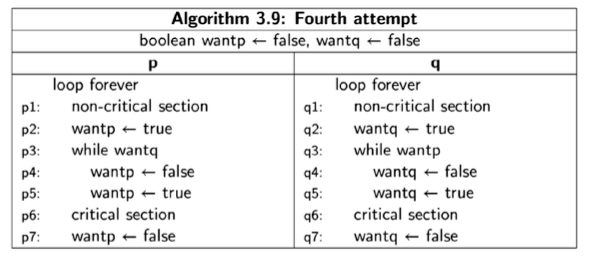
\includegraphics[width=1\textwidth]{3.9.png}\end{center}
Questo algoritmo cerca di risolvere il deadlock del 3.8 \ref{SEC:3.6} andando a resettare il valore della variabile che si riferisce al voler entrare in sezione critica qualora non si riesca ad entrare.
\subsection{Rete di Petri}
\newpage
\begin{center}
\makebox[\textwidth][c]{
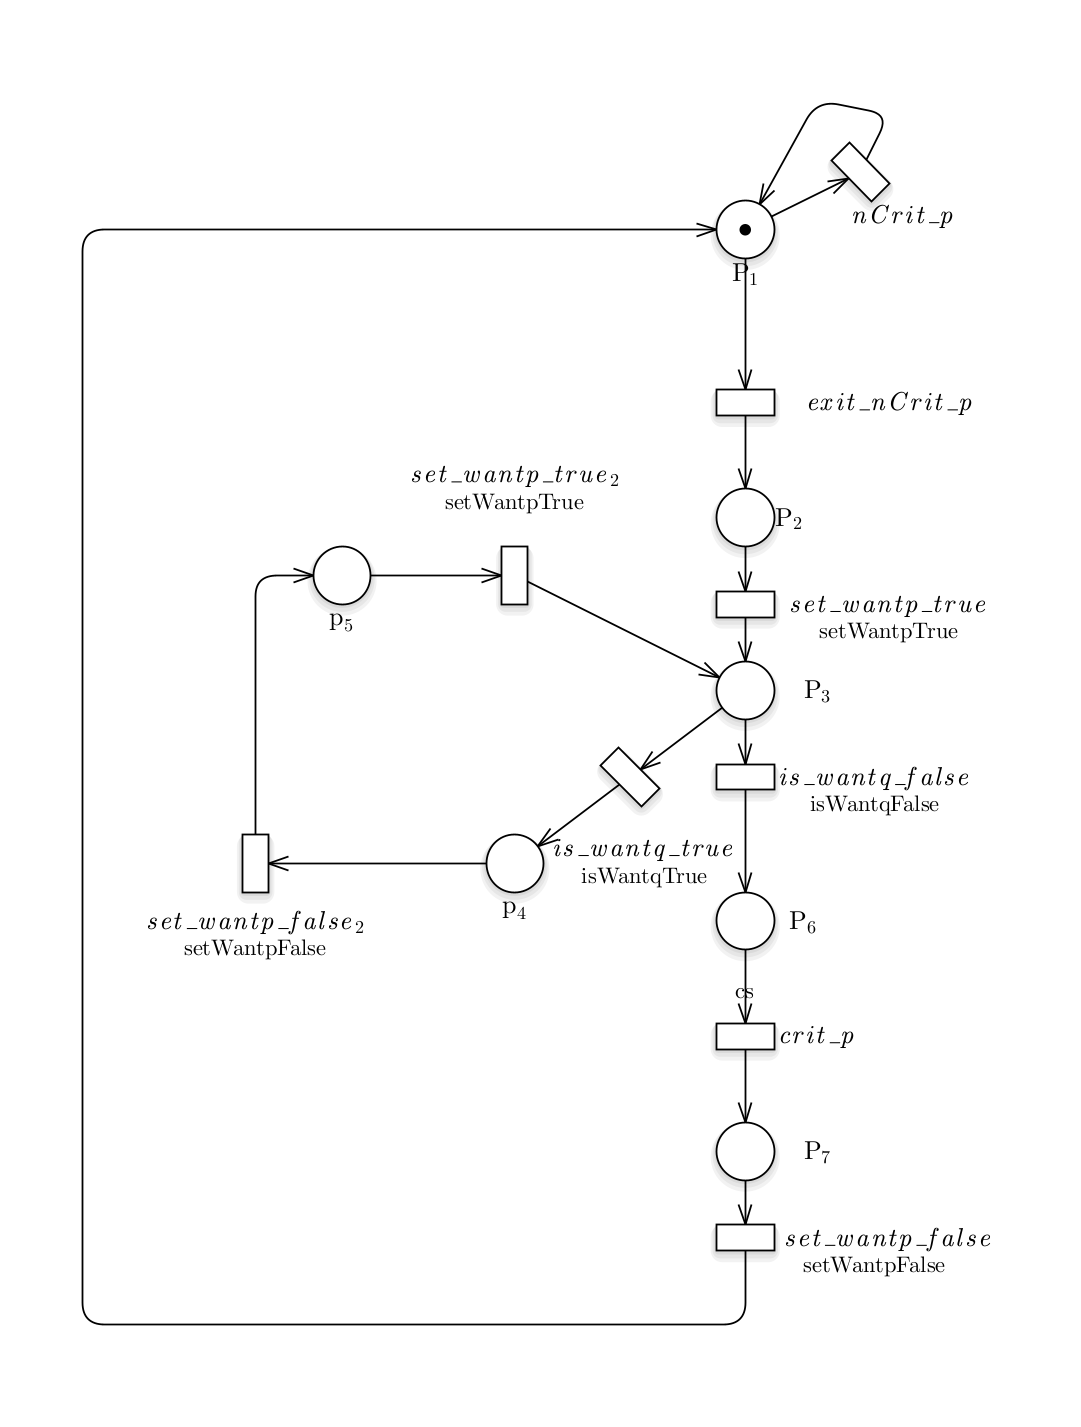
\includegraphics[width=0.4\textwidth]{p3.9.png}
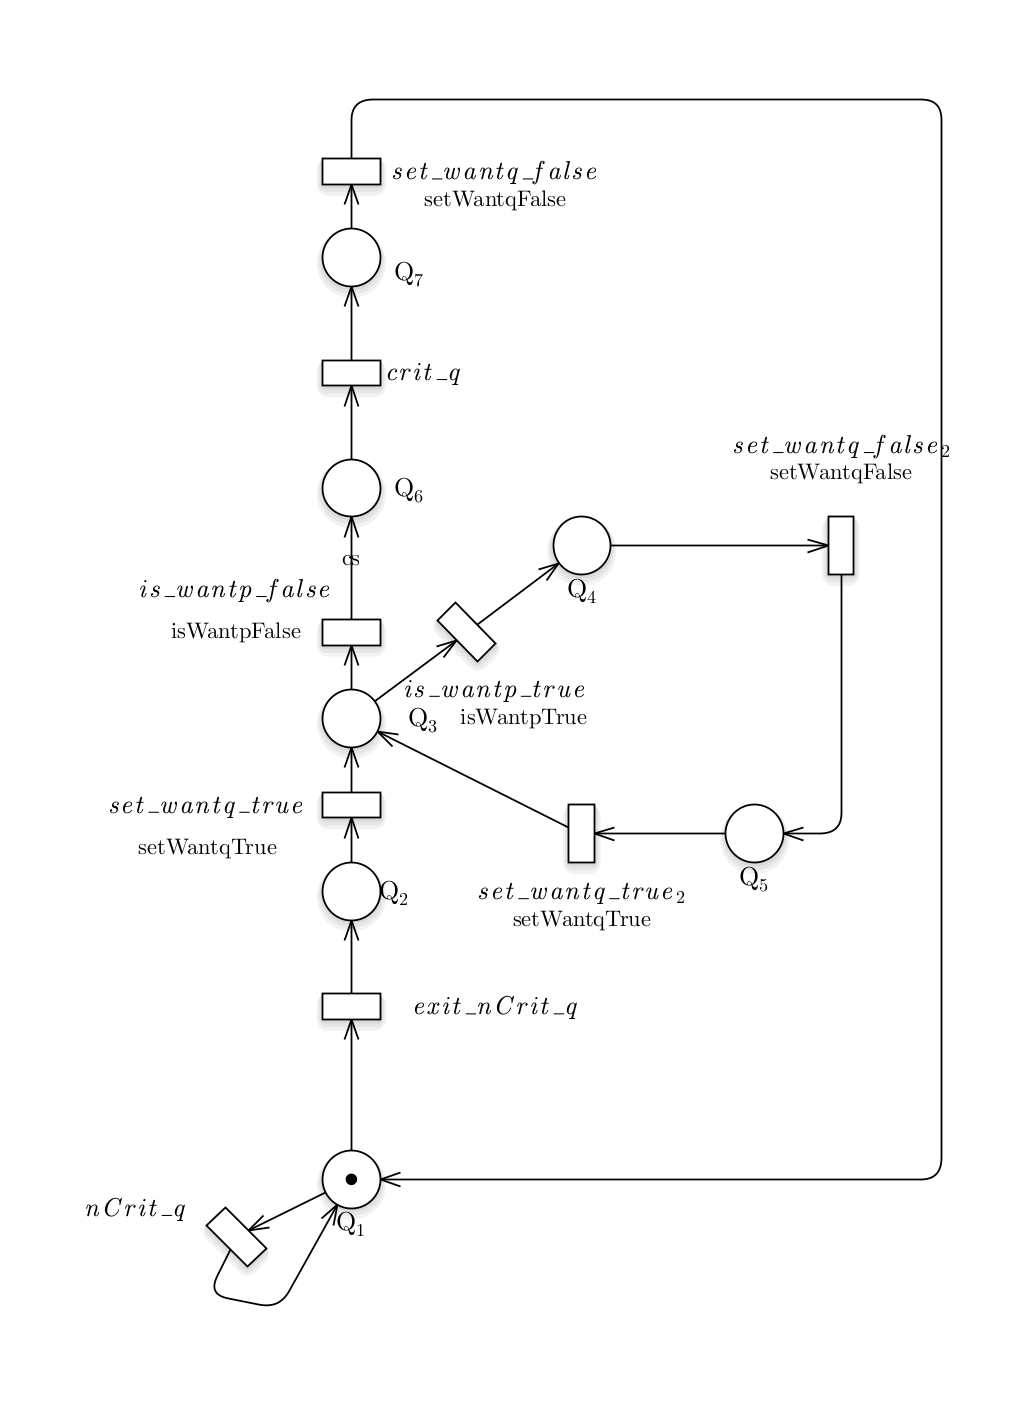
\includegraphics[width=0.4\textwidth]{q3.9.png}
}
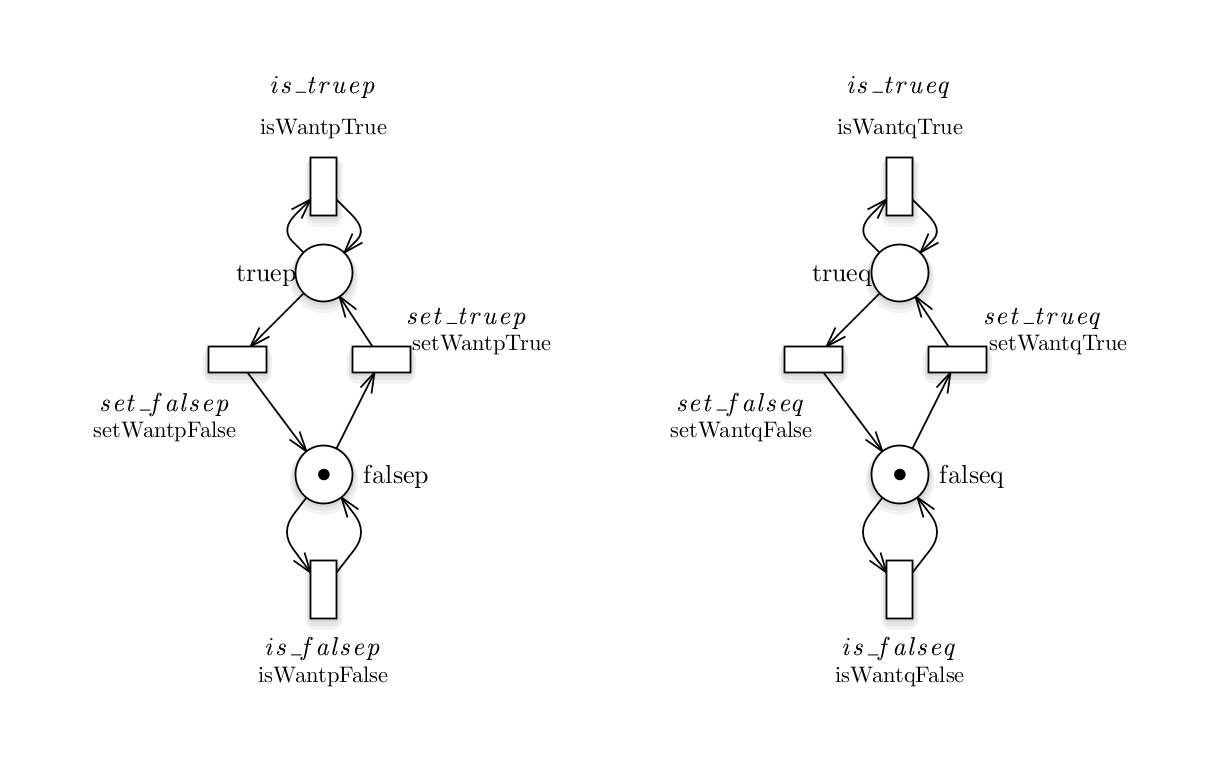
\includegraphics[width=0.8\textwidth]{variables.png}
\end{center}
\newpage
\begin{figure*}[!ht]
\centering
\makebox[\textwidth][c]{
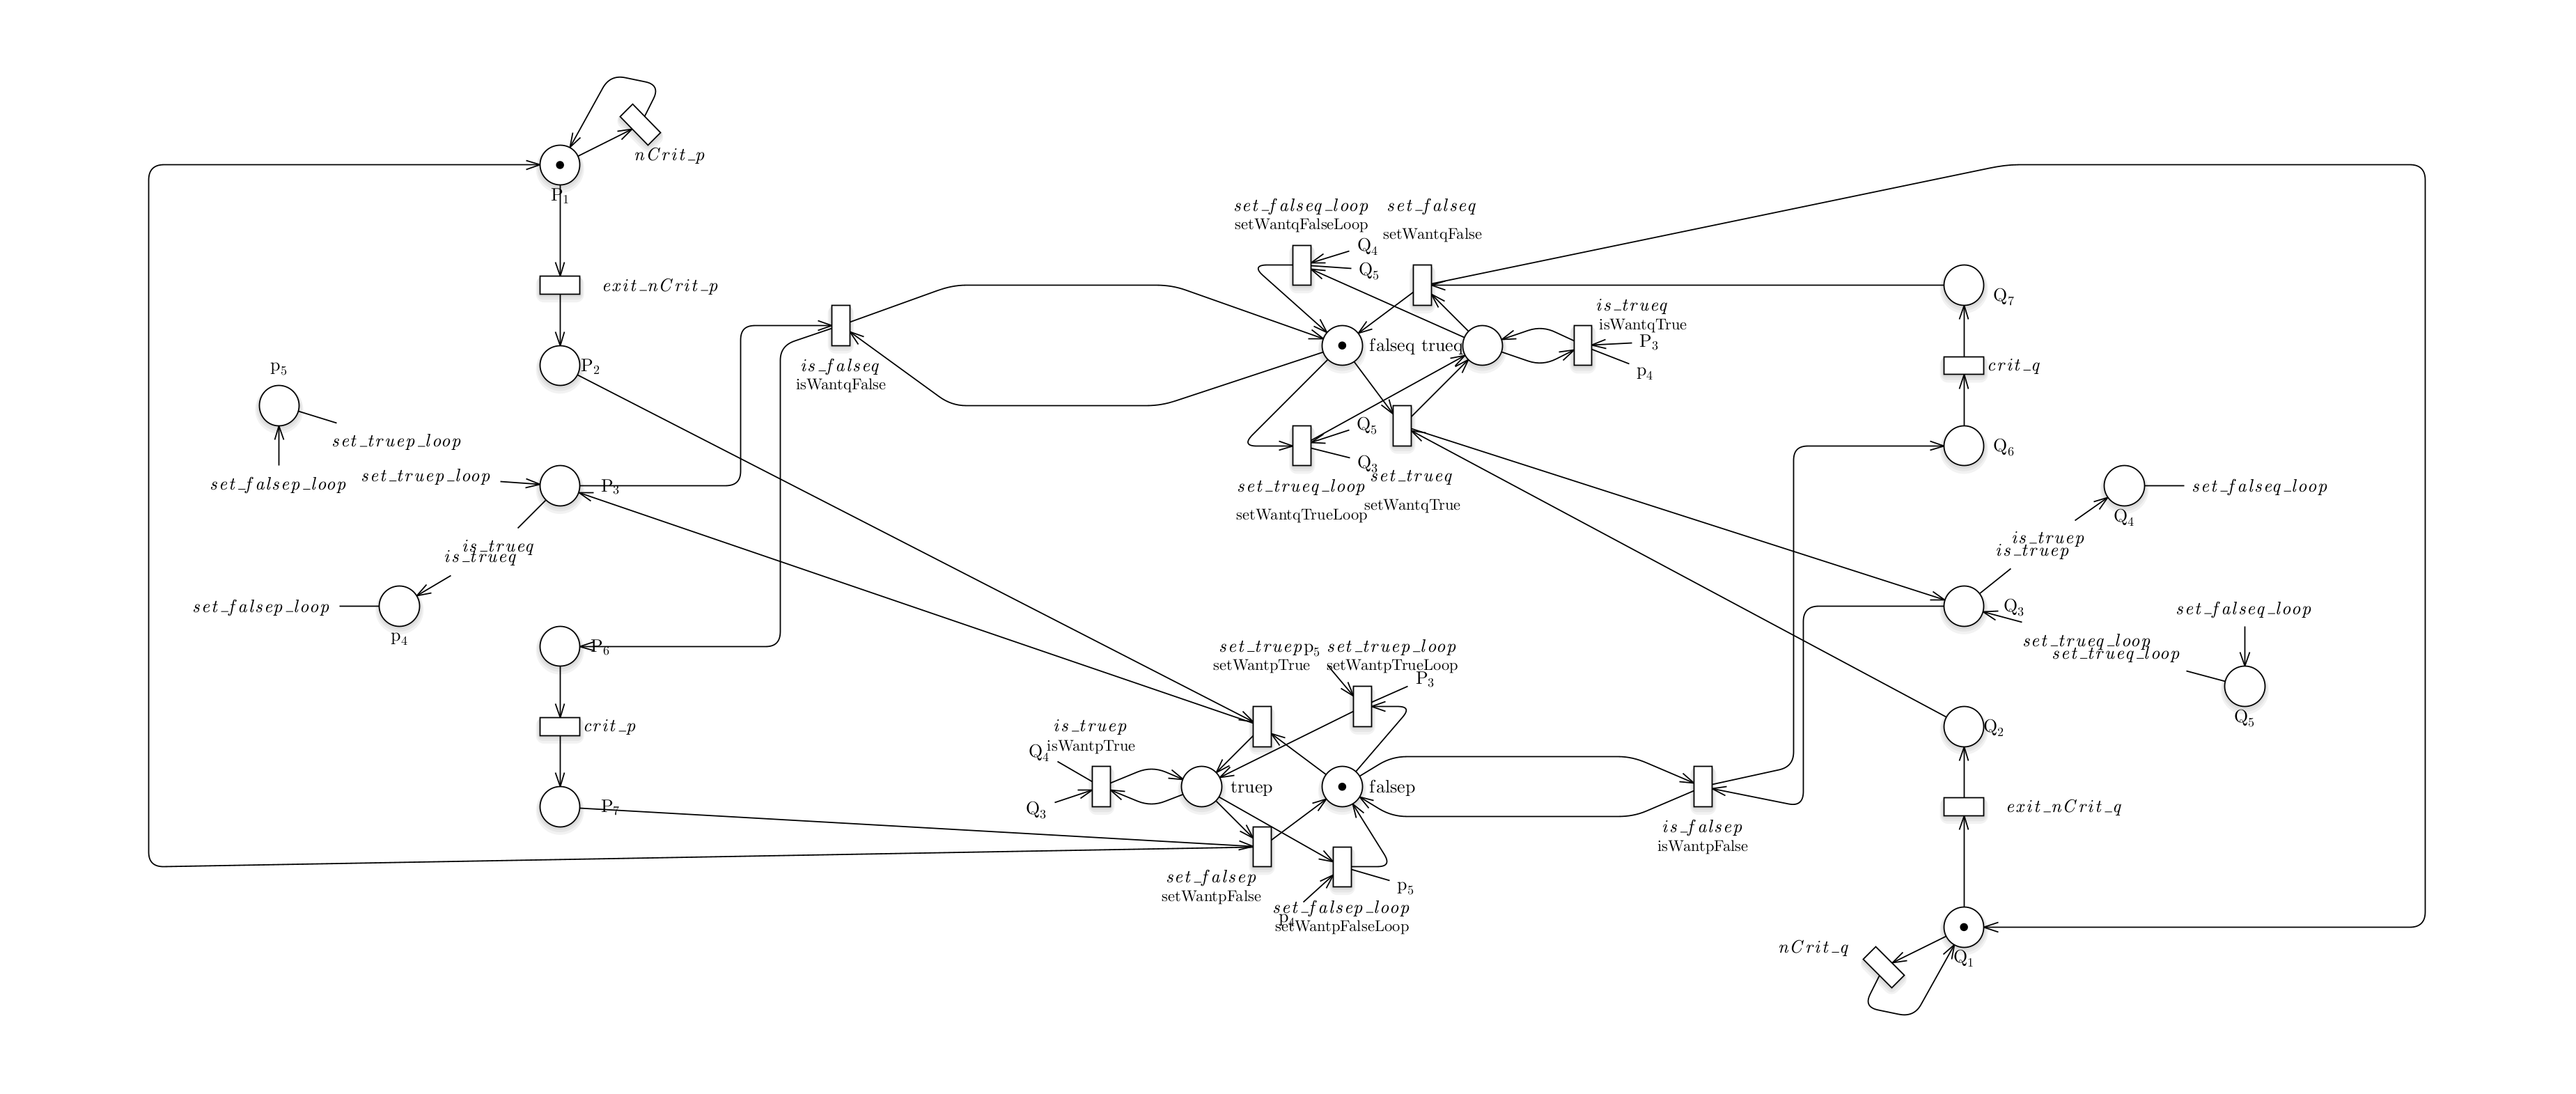
\includegraphics[width=1.6\textwidth]{3.9PN.png}}
\caption{Rete di petri composta} \label{FIG:3.9PN}
\end{figure*}
\newpage
\subsubsection{RG}
Il reachability graph, in figura \ref{FIG:3.9RG}, è composto da 45 stati, di cui nessuno rappresentante una situazione di Deadlock.
\begin{figure*}[!ht]
\centering
\makebox[\textwidth][c]{
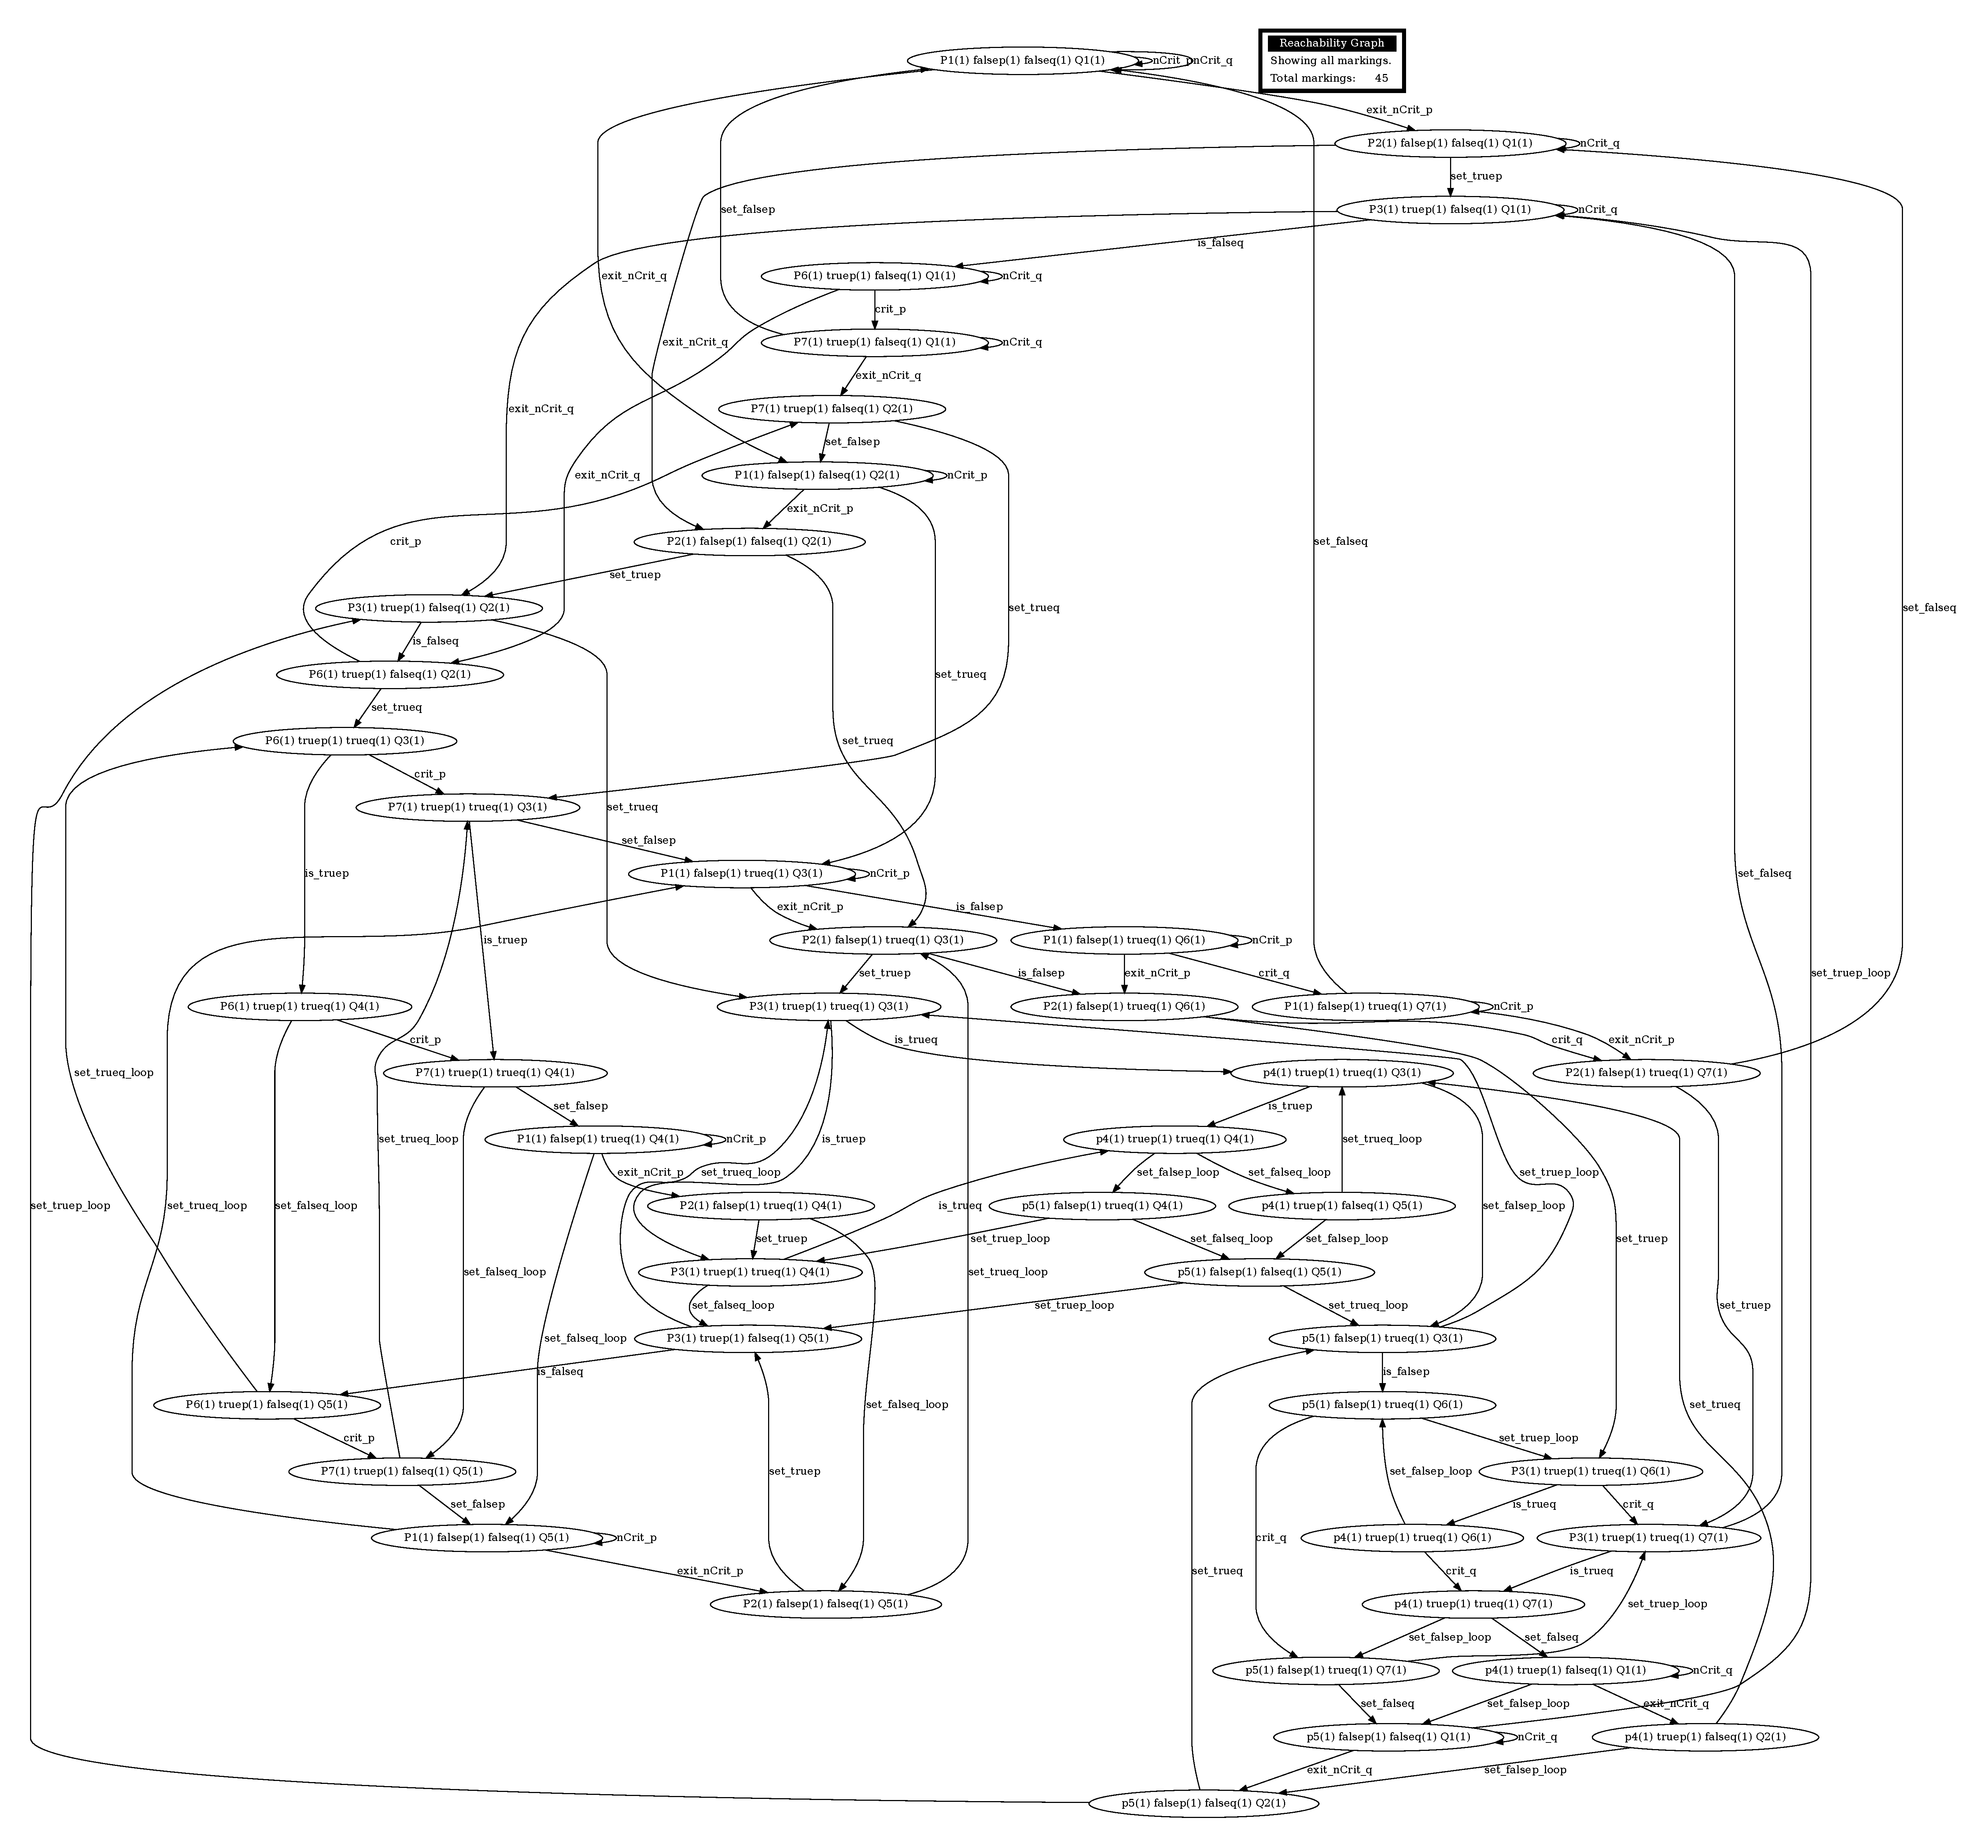
\includegraphics[width=1\textwidth]{3.9RG}}
\caption{Reachability graph 3.9} \label{FIG:3.9RG}
\end{figure*}
\newpage
\subsubsection{Analisi strutturale}

\subsubsection{Model Checking GreatSPN}
Sono state verificate le seguenti formule CTL:
\begin{itemize}
	\item mutua esclusione: \textit{AG !(\#P6==1 \&\& \#Q6==1)} \textcolor{green}{true}.\\
		Il sistema rispetta la mutua esclusione.
	\item deadlock: \textit{AG AF ((\#P1==1) || (\#Q1 == 1))} \textcolor{red}{false}.\\
		Il sistema sembra andare in deadlock, il controesempio presentato dal Model Checker è l'esecuzione in cui entrambi i processi entrano nel loop di richiesta e si bloccano a vicenda l'uscita.\\
		Ma questo non è deadlock, è starvation, quindi la formula logica usata per controllare l'assenza di deadlock in questo caso va modificata.
	\item deadlock corretto: \textit{AG AF (((\#P1==1) || (\#Q1 == 1)) || ((\#P4==1) || (\#Q4 == 1)))} \textcolor{green}{true}.\\
		In questo modo viene controllato che i processi siano liberi di eseguire o il ciclo esterno (dallo stato 1 fino al ritorno in stato 1) o almeno quello interno (dallo stato 3 ritorno allo stato 3).
	\item assenza di starvation: \textit{AG((\#P2 >0 ) -> (AF \#P6>0 ))} ed anche \textit{AG((\#P2 >0 ) -> (AF \#P6>0 ))}. Entrambe risultano \textcolor{red}{false}.\\
		Come anticipato prima si può verificare starvation. Sia perchè un processo riesce sempre ad entrare in CS escludendo l'accesso all' altro (situazione mostrata come controesempio dal Model Checker) oppure perchè entrambi i processi si bloccano a vicenda l'accesso.
\end{itemize}
Sono state verificate le seguenti formule LTL:
\begin{itemize}
	\item mutua esclusione: \textit{G !(\#P4==1 \&\& \#Q4==1)} \textcolor{green}{true}.
	\item assenza di starvation: \textit{G F (\#P2==1) -> G F(\#P6 == 1)} ed anche \textit{G F (\#Q2==1) -> G F(\#Q6 == 1)}. Entrambe risultano \textcolor{red}{false}.\\
	\item deadlock: \textit{G F( (\#P1 ==1) ||  (\#Q1 ==1))} \textcolor{red}{false}.
	\item deadlock corretto: \textit{G F ( (\#P1==1) || (\#Q1 == 1) ) || G F ((\#P4==1) || (\#Q4 == 1)))} \textcolor{green}{true}.\\
\end{itemize}

\subsection{NuSMV}
L'implementazione del sistema tramite il linguaggio di NuSMV è pressochè identica a quella della sezione \ref{SUBSEC:3.6NuSMV}, l'unica differenza sta nella posizione del controllo \texttt{!want\_other} che questa volta viene effettuato dopo aver impostato la variabile \textit{want\_me} a true.
\lstinputlisting{figures/3_9_code.smv}
Il comando \texttt{print\_reachable\_states} mostra 21 stati raggiungibili di 100 possibili, in linea con la dimensione del Reachability Graph.
È presente uno stato di deadlock : $p.state=s3, \; q.state=s3, \; wantp = true, \; wantq = true $. 

\subsubsection{Model Checking NuSMV}
Sono state verificate le seguenti formule CTL:
\begin{itemize}
        \item mutua esclusione: \textit{AG !(( p.state = s6 ) \& (q.state = s6 ))} \textcolor{green}{true}.
        \item deadlock: \textit{AG AF (( p.state = s1 )| ( q.state = s1 ))} \textcolor{red}{false}.\\
		Si verifica di nuovo la stesso situazione presentata in GreatSPN, la formula è incorretta per verificare l'assenza di deadlock. Va quindi riscritta.

        \item deadlock: \textit{AG AF ((( p.state = s1 ) | ( q.state = s1 ) ) | (( p.state = s4 ) | ( q.state = s4 ) ))} \textcolor{green}{true}.\\
        \item assenza di starvation: \textit{AG (( p.state = s2 ) -> (AF p.state = s3 ))} ed anche \textit{AG (( q.state = s2 ) -> (AF q.state = s3 ))}. Entrambe risultano \textcolor{red}{false}.\\
		Come visto nel Model Checking in GreatSPN si può verificare starvation sia perchè un processo blocca l'altro e va solo lui in critical section ma anche perchè entrambi si bloccano l'accesso a vicenda.
		Il controesempio fornito dal MC è una istanza del secondo tipo.
\end{itemize}
Sono state verificate le seguenti formule LTL:
\begin{itemize}
        \item mutua esclusione: \textit{G !(p.state = s4 \& q.state = s4)} \textcolor{green}{true}.\\
        \item deadlock: \textit{G F(( p.running) | ( q.running ) )} \textcolor{green}{true}. \\
		In questo caso il problema di definizione della formula logica "il processo può essere eseguito" non si pone, in quanto NuSMV permette di utilizzare la clausola \texttt{running} per stabilire se un processo sta venendo eseguito o no (questo solo il LTL).\\
		Quindi il Model Checker mostra correttamente l'assenza di Deadlock.
        \item assenza di starvation: \textit{G (p.state = s2 ->  F p.state = s3)} ed anche \textit{G (p.state = s2 ->  F p.state = s3)}. Entrambe risultano \textcolor{red}{false}.\\
		Essendoci deadlock c'è sempre la possibilità di starvation. Se il sistema va in deadlock dopo l'esecuzione presentata precedente entrambi i processi presentano starvation.
		L'esempio presentato dal Model Checker è lo stesso del caso di deadlock.
\end{itemize}


\end{document}
